Having introduced the theoretical foundations of machine learning and the specific architecture of the Transformer model used in this work, we now turn to their practical implementation in the context of this work. 
This chapter begins by outlining the structure and organization of waveform data in the LEGEND-200 experiment. We then describe the procedure for constructing training datasets, which includes data selection and data cleaning. 
The different models developed in this work are presented alongside their classification performance. We continue with a brief overview of the pulse shape simulation (PSS) framework in LEGEND-200, and conclude this chapter by summarizing key results. 


\subsection{Data in the LEGEND-200 experiment} \label{sec:04_LEGEND_data}

The DAQ process in LEGEND-200 follows a structured hierarchy to ensure consistency across the dataset. Each DAQ cycle -- a continuous block of data-taking, synchronously started and stopped by the DAQ system -- is stored as a separate file and marked with a GPS timestamp.  
A sequence of DAQ cycles recorded under a consistent detector configuration is grouped into a run. Each run begins with a series of calibration cycles, followed by physics cycles. 
Runs are then grouped into larger units called periods, which are separated by major changes in the detector setup or operating conditions that could impact analysis results. 
However, not all periods and runs are suitable for physics analysis. Only a subset has passed the data quality checks established by the collaboration~\cite{lnote_24010}. Table~\ref{tab:periods_runs} summarizes all physics runs that were deemed usable for this work.

\begin{table}[b]
\centering
\caption{Summary of all physics runs that passed the LEGEND quality checks~\cite{lnote_24010}, including live time and total exposure (ICPC detectors only). } 
\begin{tabular}{||c | c | c| c | c||} 
    \hline
    \textbf{Period} & \textbf{Runs} & \textbf{Start date} & \textbf{Live time [yr]}  & \textbf{Exposure [kg$\cdot$yr]} \\ 
    \hline
    3 & 0-5 & 2023-03-12 & 0.08 & 4.85 \\
    \hline
    4 & 0-3 & 2023-04-15 & 0.047 & 2.89 \\
    \hline
    6 & 0-5 & 2023-06-11 & 0.110 & 6.68 \\
    \hline
    7 & 2-7 & 2023-07-31 & 0.096 & 5.82 \\
    \hline
    8 & 0-4, 6-14 & 2023-10-03 & 0.237 & 14.39 \\
    \hline
    9 & 0-5 & 2024-01-11 & 0.093 & 5.67 \\
    \hline
\end{tabular}
\label{tab:periods_runs}
\end{table}

The raw waveforms recorded by the LEGEND-200 experiment are stored at NERSC in HDF5 (Hierarchical Data Format version 5). HDF5 is a binary file format designed to store and organize large, complex datasets. It is well-suited for large datasets because it supports fast I/O and efficient partial data access. Therefore, the entire file need not be loaded into memory. 

The collaboration has developed a sophisticated digital signal processing pipeline. Its initial stage operates directly on the raw waveforms, with subsequent stages performing higher-level processing, as illustrated in figure~\ref{fig:data_flow}. 

In the initial stage, the digitized waveforms recorded by the DAQ system are stored in the RAW (raw waveform and ADC information) tier. This tier also includes metadata such as the timestamp of the recording and the measured energy in ADC units. 
For the DSP (digitally processed features)  tier, each waveform is processed independently to extract signal features. This tier contains several parameters directly derived from the waveform, for example, various energy estimates, amplitude, and baseline. 
The HIT (hit-level calibrated parameters) tier contains parameters derived from a multi-waveform analysis. This includes calibrated energy values, A/E ratios, and LQ cut values. All data tiers up to this point are organized in separate subdirectories and indexed by timestamp, enabling efficient access to specific waveforms. 
In contrast, the EVT (event cluster level) tier clusters individual waveforms into events. Each event may consist of multiple coincident hits in the HPGe detectors, as well as in other subsystems, such as the SiPMs and the muon veto. 
Finally, the TCM (trigger and calibration metadata) tier includes information related to event building, along with data from calibration pulses.


\begin{figure}[t]
    \centering
    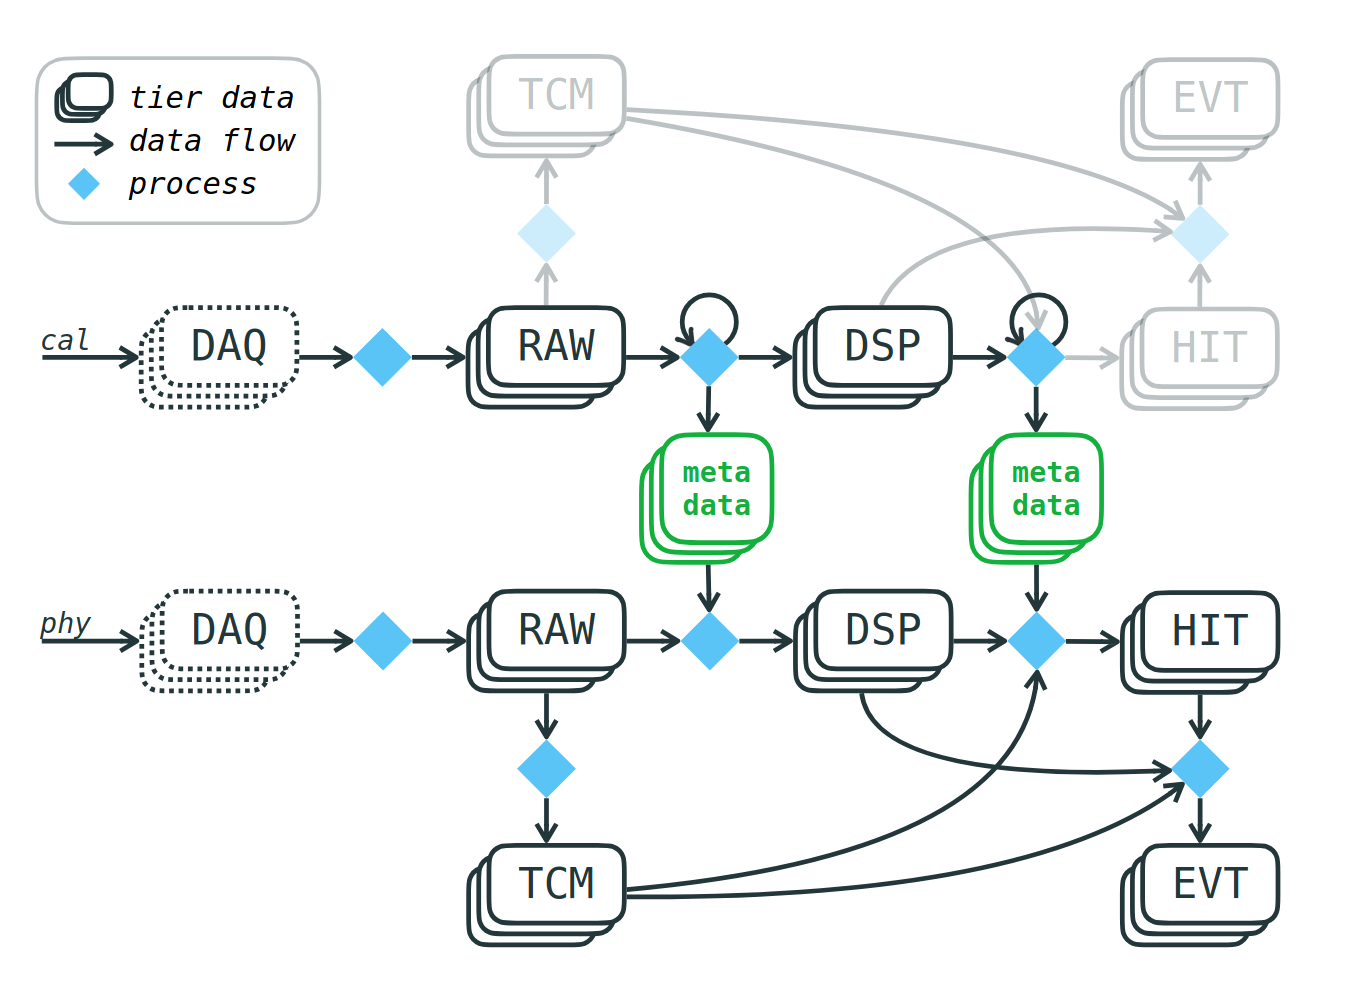
\includegraphics[width=0.85\linewidth]{figures/05_PSD/Data_flow.png}
    \caption{Data flow for the LEGEND-200 experiment. Starting from the DAQ output, the data undergoes multiple processing steps before being clustered into coincident events in the EVT tier. The calibration data, acquired using sources that produce signals at well-known energies, is used to define and validate analysis cuts and to establish a precise energy scale. These calibrations are then applied to the physics data. Image credit to Luigi Pertoldi~\cite{noauthor_pyhep_2023}. } 
\label{fig:data_flow}
\end{figure}


\subsection{Data preparation for Transformer training}

In supervised machine learning, the quality of the training data is critical. The performance of a model is fundamentally limited by the cleanliness and reliability of the dataset it is trained on. 

To address this, we developed a code framework that combines waveforms and processing parameters from multiple data tiers into a unified dataset suitable for training machine learning models. Each waveform is then classified (labeled) according to the established LEGEND-200 analysis methods. 

The dataset is subsequently cleaned to maximize class purity and minimize contamination from misclassified events. The impact of this data-cleaning procedure is illustrated in figure~\ref{fig:datacleaning_fullspectrum}, where we show data from period 3 (only ICPC detectors).

\begin{figure}[t]
    \centering
    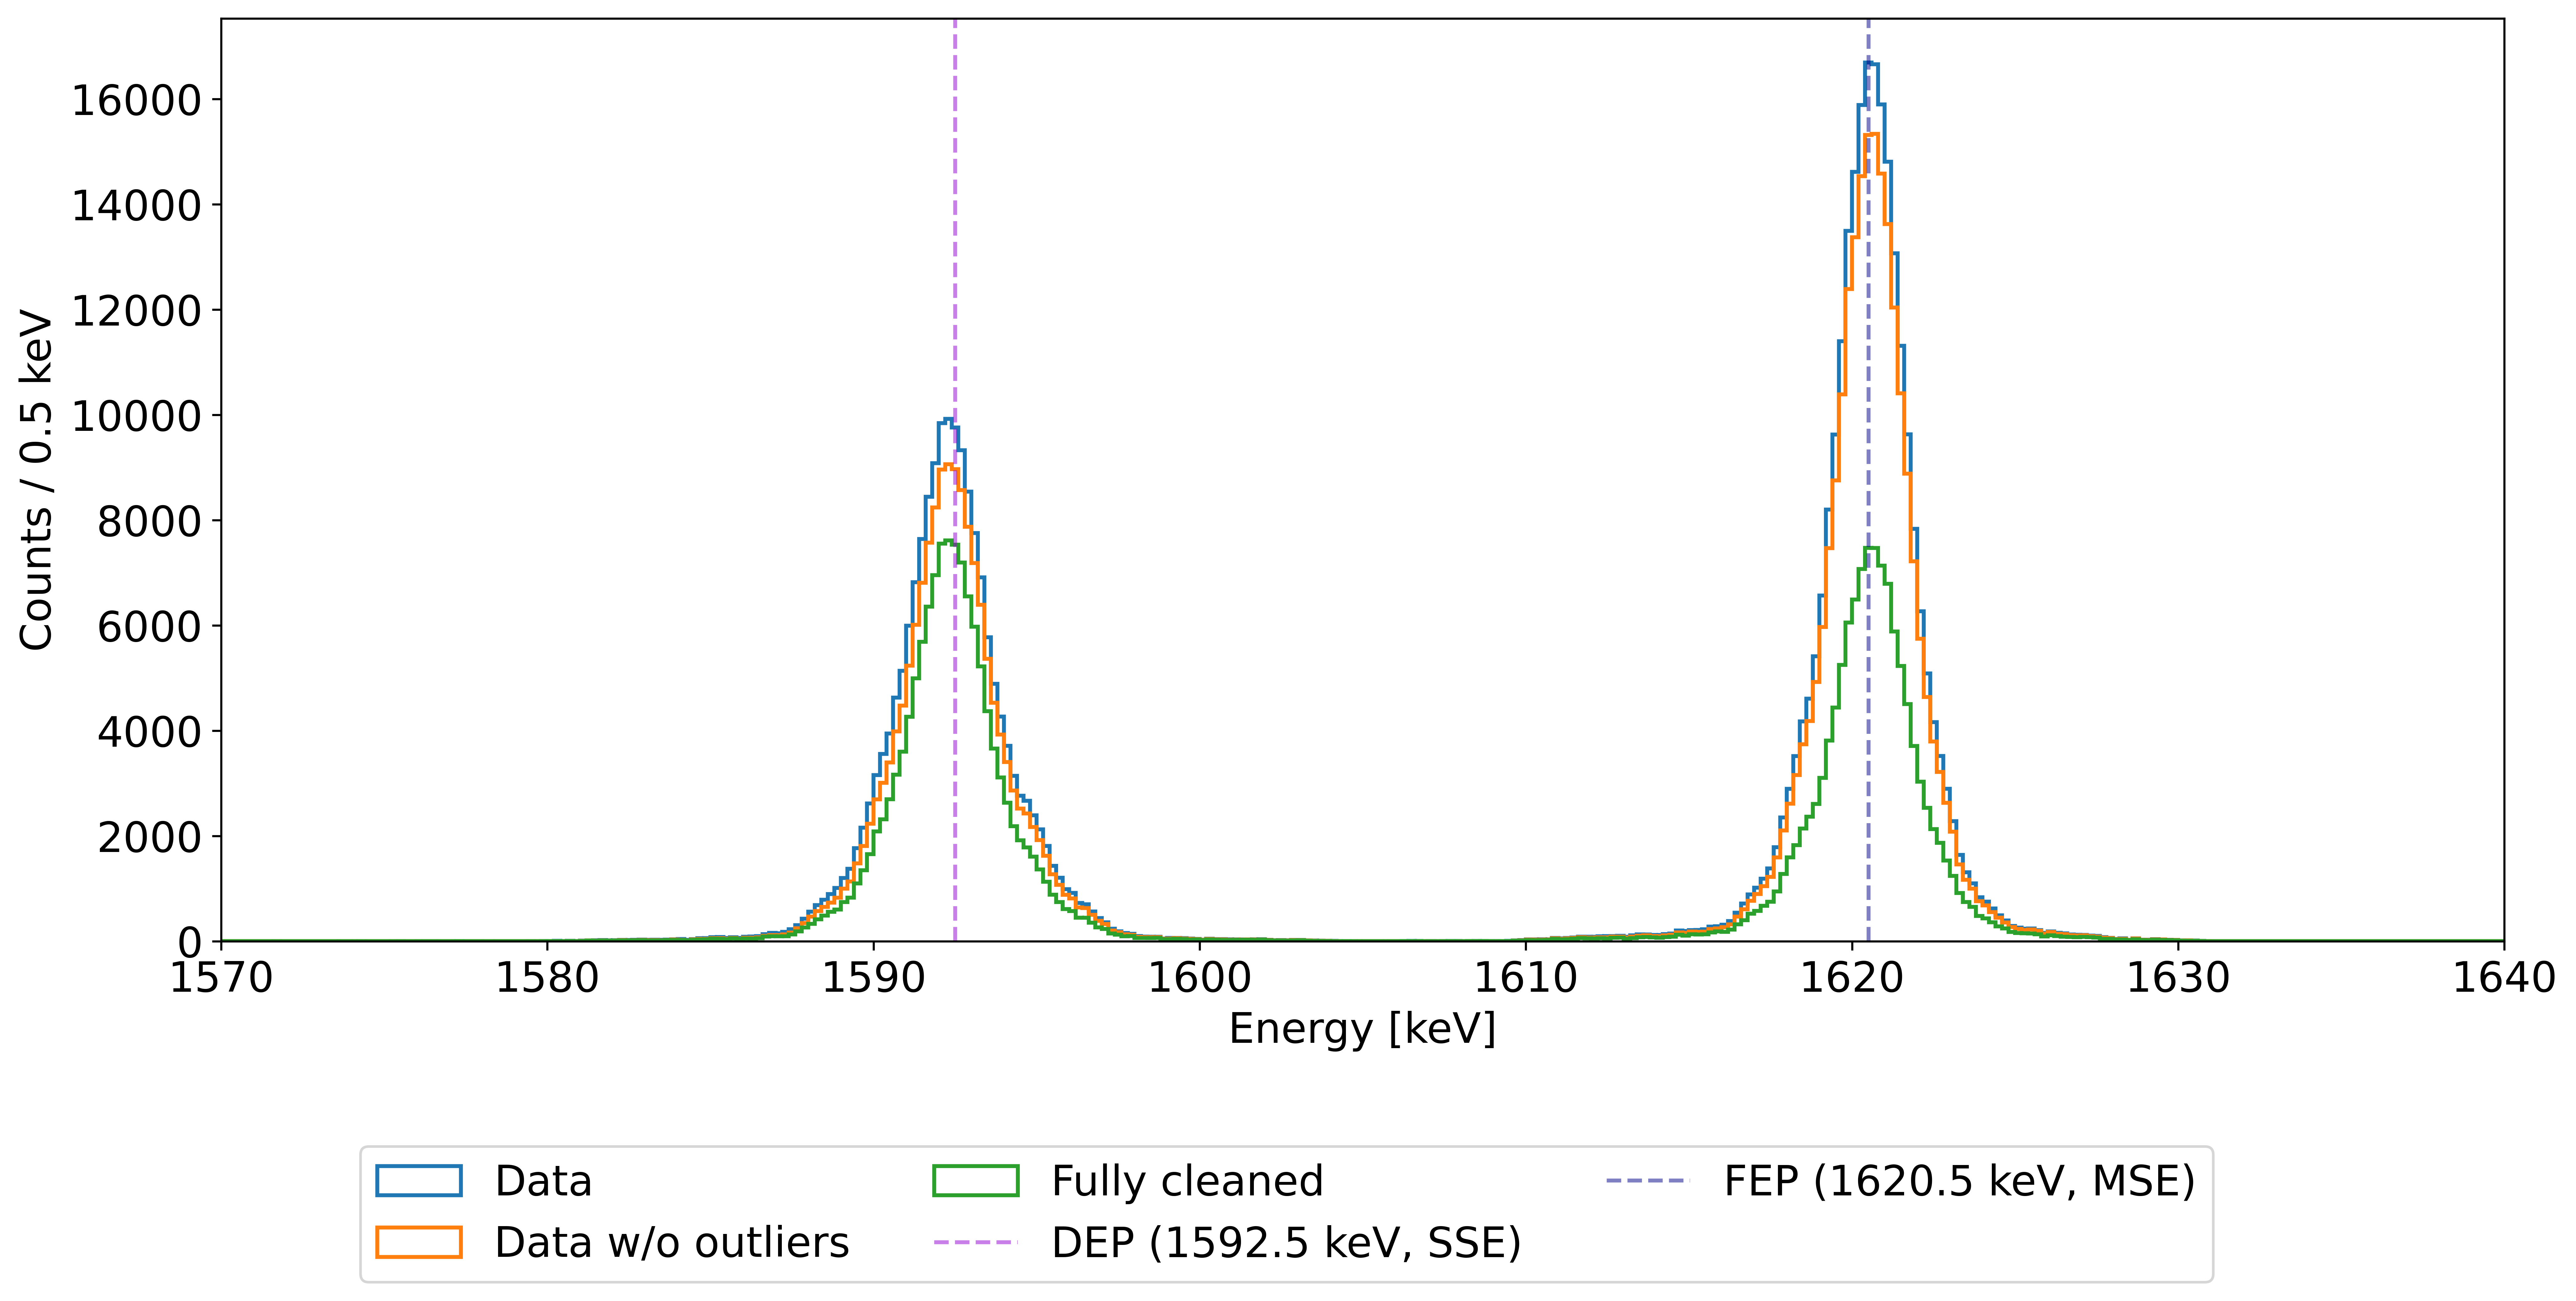
\includegraphics[width=\linewidth]{figures/05_PSD/Data_cleaning_fullspectrum.png}
    \caption{Effect of the data cleaning procedure on two pre-selected peaks ($\pm 3\, \sigma$) from the $^{228}$Th calibration in period 3, using only ICPC detectors. The plot shows the impact of the two cleaning steps applied to pre-selected data (blue): removal of statistical outliers (orange) and exclusion of events with non-matching numbers of peaks in the gradient waveforms (green, combined effect). The latter has a strong impact on the full energy peak, as expected, since SSEs are already very pure, while the MSE class tends to be heterogeneous.} 
\label{fig:datacleaning_fullspectrum}
\end{figure}


\subsubsection{Data selection}

The data selection begins by loading the calibrated energies from the HIT tier. In this work, we use the energy estimated with the trapezoid filter (explained in section~\ref{sec:HPGe_legend}). The HDF5 files, which have a specific structure, are accessed with \textit{legend-pydataobj}, a package that provides a Python implementation of the LEGEND Data Objects to HDF5~\cite{detwiler_legend-pydataobj_2025}. Detector metadata is used to select only detectors that were active and functioning properly during data taking. 

For events falling within a specified energy range, the corresponding indices are stored for further processing. For datasets intended for training, the algorithm automatically selects a $ \pm 3 \,\sigma$ window around the four prominent calibration peaks in the $^{228}$Th spectrum. 
This window is estimated from the FWHM of the energy resolution. Alternatively, a custom energy window can be manually defined, for example, to load a continuous dataset for benchmarking the Transformer model against conventional PSD methods. 
Once the energy range is specified, waveforms are loaded from the RAW tier by indexing the file location within the subdirectory structure. Throughout this work, we use waveforms windowed around the rising edge, sampled 1400 times at 16~ns intervals. 
Pre-selecting events in the HIT tier significantly reduces runtime by up to two orders of magnitude, since only waveforms in the relevant energy range are loaded. These energy windows typically span tens of keV and represent only a small fraction of the total dataset. 

We then apply quality cuts to remove waveforms that deviate from expected detector response characteristics. For this purpose, we apply the same set of quality cuts developed and validated for the LEGEND-200 physics analyses, which are defined in~\cite{lnote_24011}. We remove all waveforms that contain:

\begin{itemize}
    \item discharges (is\_delayed\_discharge)
    \item unstable baselines (is\_valid\_bl\_slope, is\_valid\_bl\_slope\_rms)
    \item noisy tails (is\_valid\_tail\_rms)
    \item noise bursts in the rising edge (is\_not\_noise\_burst)
    \item invalid energies (is\_valid\_cuspEmax, is\_valid\_cuspEmin, is\_low\_cuspEmax)
    \item invalid trap filter (is\_valid\_trap\_tpmin, is\_valid\_trap\_tpmax)
    \item invalid rise times (is\_valid\_t0, is\_valid\_rt, is\_valid\_dteff)
\end{itemize}

In the final step of the data selection, the remaining events are classified.
As discussed in section~\ref{sec:02_PSD} and shown in figure~\ref{fig:PSD_topology}, the amplitude-to-energy ratio is particularly well suited for distinguishing different event topologies. Table~\ref{tab:event_classification} summarizes the classification scheme. 

The resulting dataset consists of waveforms within the desired energy range that have been classified accordingly. While the class labels are already very pure, the events within each class still exhibit a degree of heterogeneity that will affect model training. 

\begin{table}
\centering
\caption{Analytical labels for the waveforms, based on the LEGEND-200 analysis. The most important component is the A/E parameter. For ICPC detectors produced by Mirion Technologies, the LQ cut is not applied because it is not reliable.} 
\begin{tabular}{||c | c | c||} 
 \hline
 \textbf{Label} & \textbf{A/E value} & \textbf{LQ value} \\ 
 \hline
 SSE & intermediate & low \\ 
 \hline
 MSE & low & - \\ 
 \hline
 p-contact & high & - \\ 
 \hline
 n-contact & low & high \\ 
 \hline
\end{tabular}
\label{tab:event_classification}
\end{table}

\subsubsection{Data cleaning}

In the second stage of the data preparation, the dataset is further cleaned to increase the purity of the class labels. Two methods are applied: peak estimation and outlier removal. 
For peak estimation, the derivative of each waveform is computed. To increase the robustness of the peak identification, the gradients are smoothed using a rolling window with a Gaussian kernel (applied over 5 timestamps with a width of $1.5 \,\sigma$). The resulting derivative signal is then normalized to reduce energy dependence. 



To identify distinct signal components in the derivative waveform, we used the \textit{find\_peaks} function from the scipy module~\cite{virtanen_scipy_2020}, which allows for peak detection based on height and prominence. An example of single-site and multi-site peak identification is shown in figure~\ref{fig:datacleaning_PeakID}. 
For waveforms labeled as MSE, multiple peaks are required, as this corresponds to multiple time-separated charge drifts within a germanium diode. For all other event categories, only a single peak per waveform is permitted. 
Note that the labels of the waveforms are not changed during this process; instead, waveforms that do not meet the peak criteria are simply rejected. This cleaning cut is very strict, and removes more than half of the events ($51.2~\%$, benchmarked on period 3). In this step, we also extract the FWHM of the largest peak, which is used for outlier rejection.

\begin{figure}[t]
    \centering
    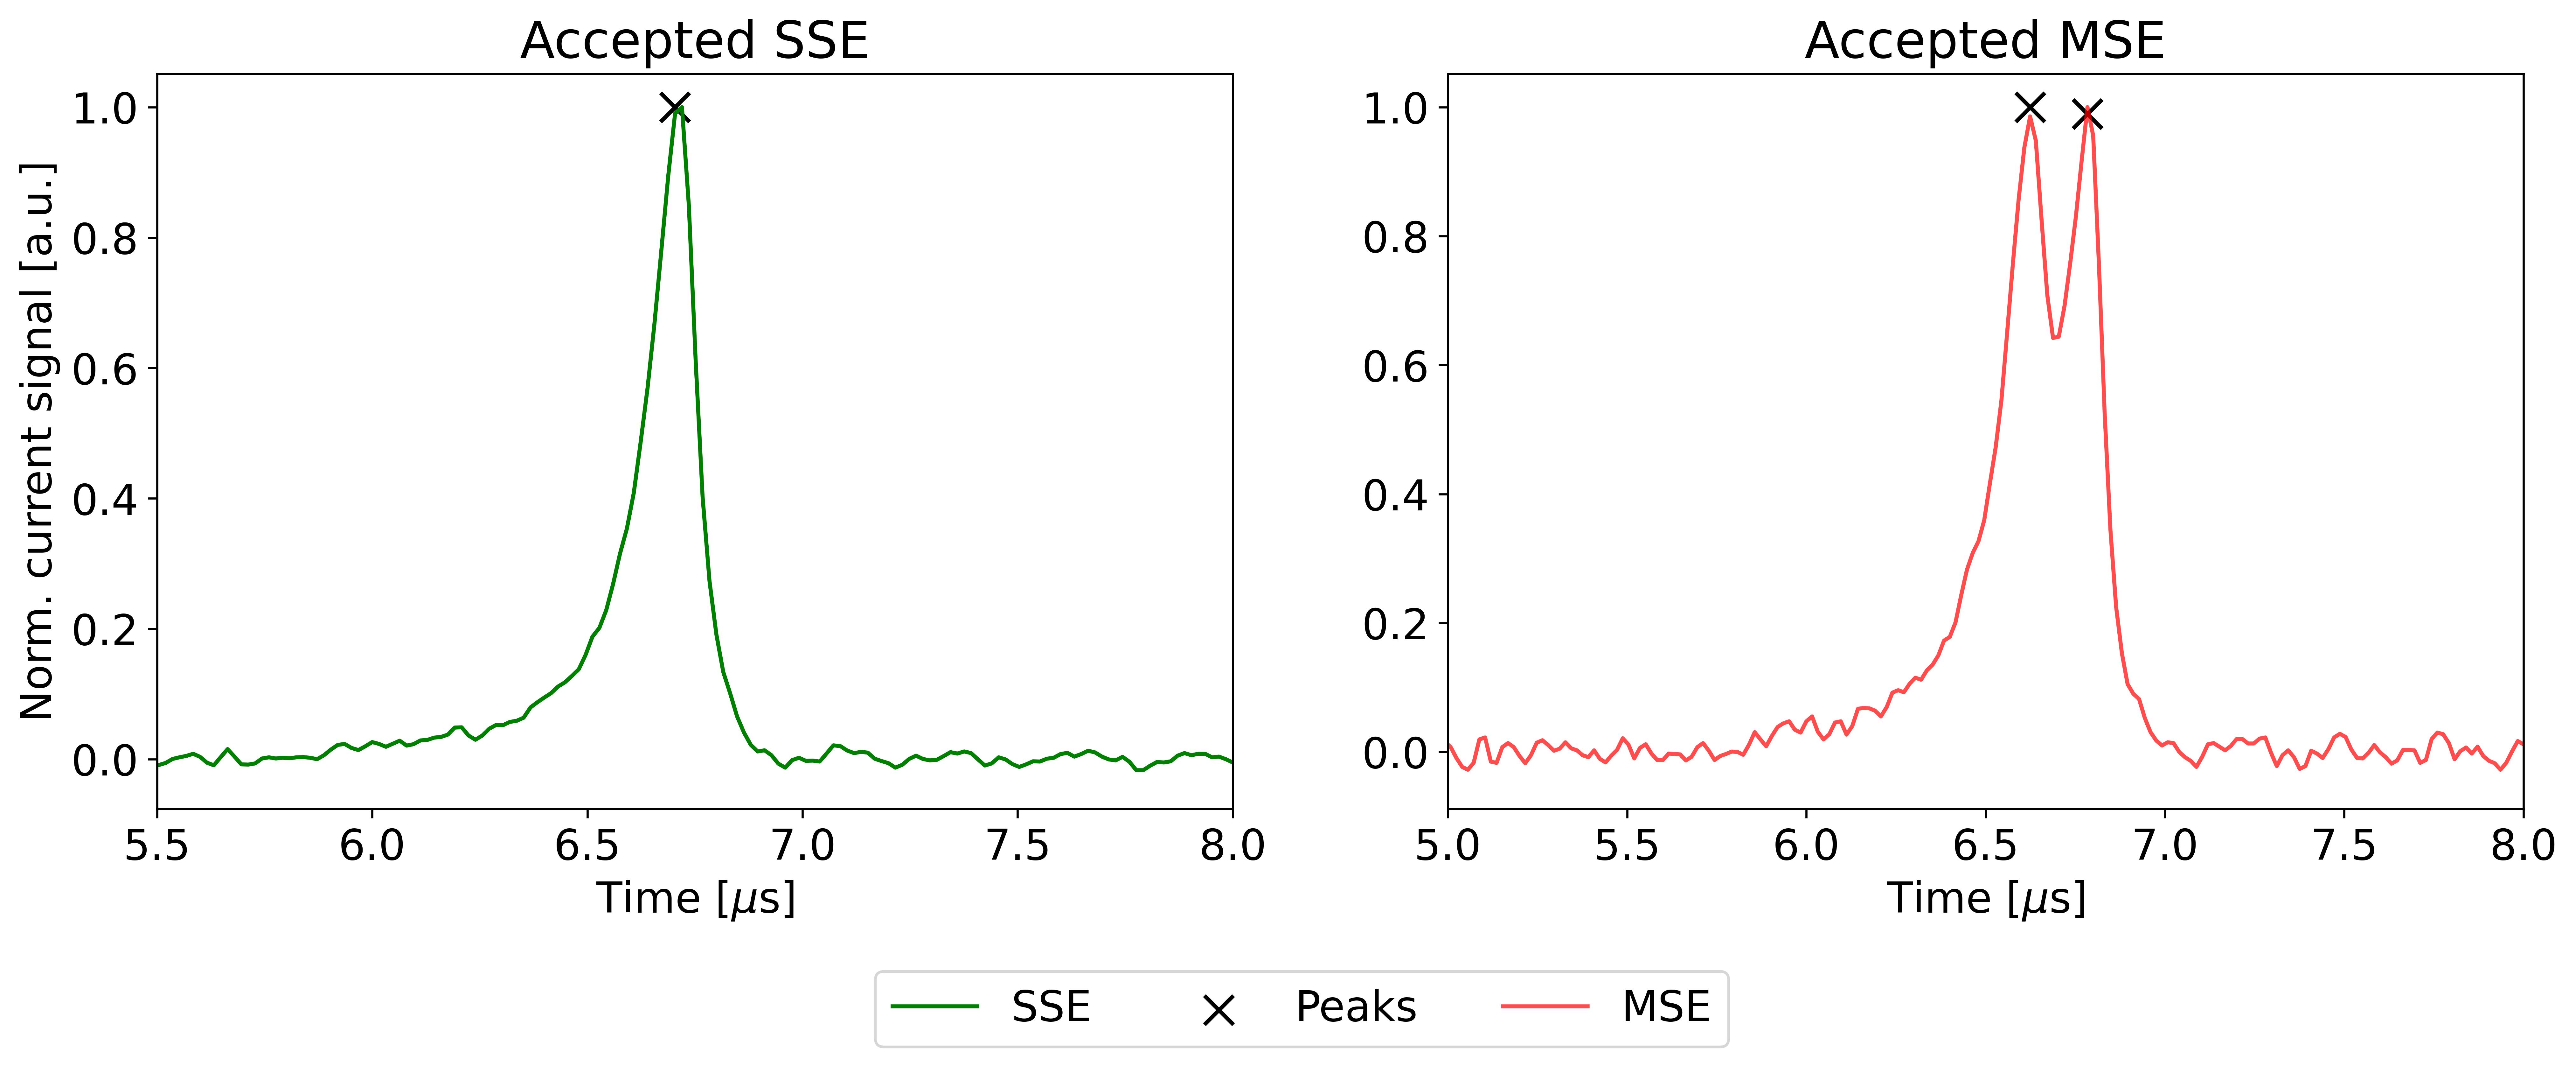
\includegraphics[width=\linewidth]{figures/05_PSD/Plot_DataCleaning_PeakID_V02160A.png}
    \caption{Peak identification for ICPC detector V02160A during period 3. The left panel shows a single-site event with one identified peak; the right panel shows a multi-site event with multiple peaks. Both are accepted.}
\label{fig:datacleaning_PeakID}
\end{figure}

\begin{table}
\centering
\caption{Parameters where outliers are removed in the data cleaning procedure. Generally, only a few events are removed in each cut ($< 3\%$). Efficiency values are determined from data taken during period 3. The total efficiency is obtained by applying all cuts simultaneously and is smaller than the product of individual efficiencies, as some waveforms fail multiple cuts. }
\begin{tabular}{||c | c | c | c |c ||} 
 \hline
 \textbf{Quantity} & \textbf{Description} & \textbf{Range} & \textbf{Cut Eff.} [\%] \\ 
 \hline
 tp-10 & Time where $A$ reaches 10 \%  	& $3 \,\sigma$ & 97.7\\ 
 \hline
 tp-50 & Time where $A$ reaches 50 \% 	& $3 \,\sigma$ & 98.0 \\ 
 \hline
 tp-80 & Time where $A$ reaches 80 \% 	& $3 \,\sigma$ & 97.8 \\
 \hline
 rt1 & Time between tp-10 and tp-90 				& $3 \,\sigma$ & 97.8 \\
 \hline
 rt2 & Time between tp-10 and tp-50 				& $3 \,\sigma$ & 97.6 \\ 
 \hline
 AoE & Area divided by energy & $3 \,\sigma$ & 99.0 \\
 \hline
 LQ & Measure for the late charge 			& $3 \,\sigma$ & 99.1 \\
 \hline
 Peak width & FWHM of the largest peak 		& $2 \,\sigma$ & 98.0 \\
 \hline
 \textbf{Total} & All cleaning cuts applied & - & 91.9 \\
 \hline
\end{tabular}
\label{tab:Data_cleaning_param}
\end{table}

To identify outliers, we calculate the mean and standard deviation of all parameters listed in table~\ref{tab:Data_cleaning_param}, separately for each detector and label. Waveforms with a peak FWHM outside a $ \pm 3 \,\sigma$ window are rejected -- except for MSE events, where we apply only a lower-bound cut. 
This exception accounts for cases where two nearby peaks merge slightly, causing the FWHM of the dominant peak to broaden. Such events are not rejected to preserve valid MSE samples. 

\begin{figure}[t]
    \centering
    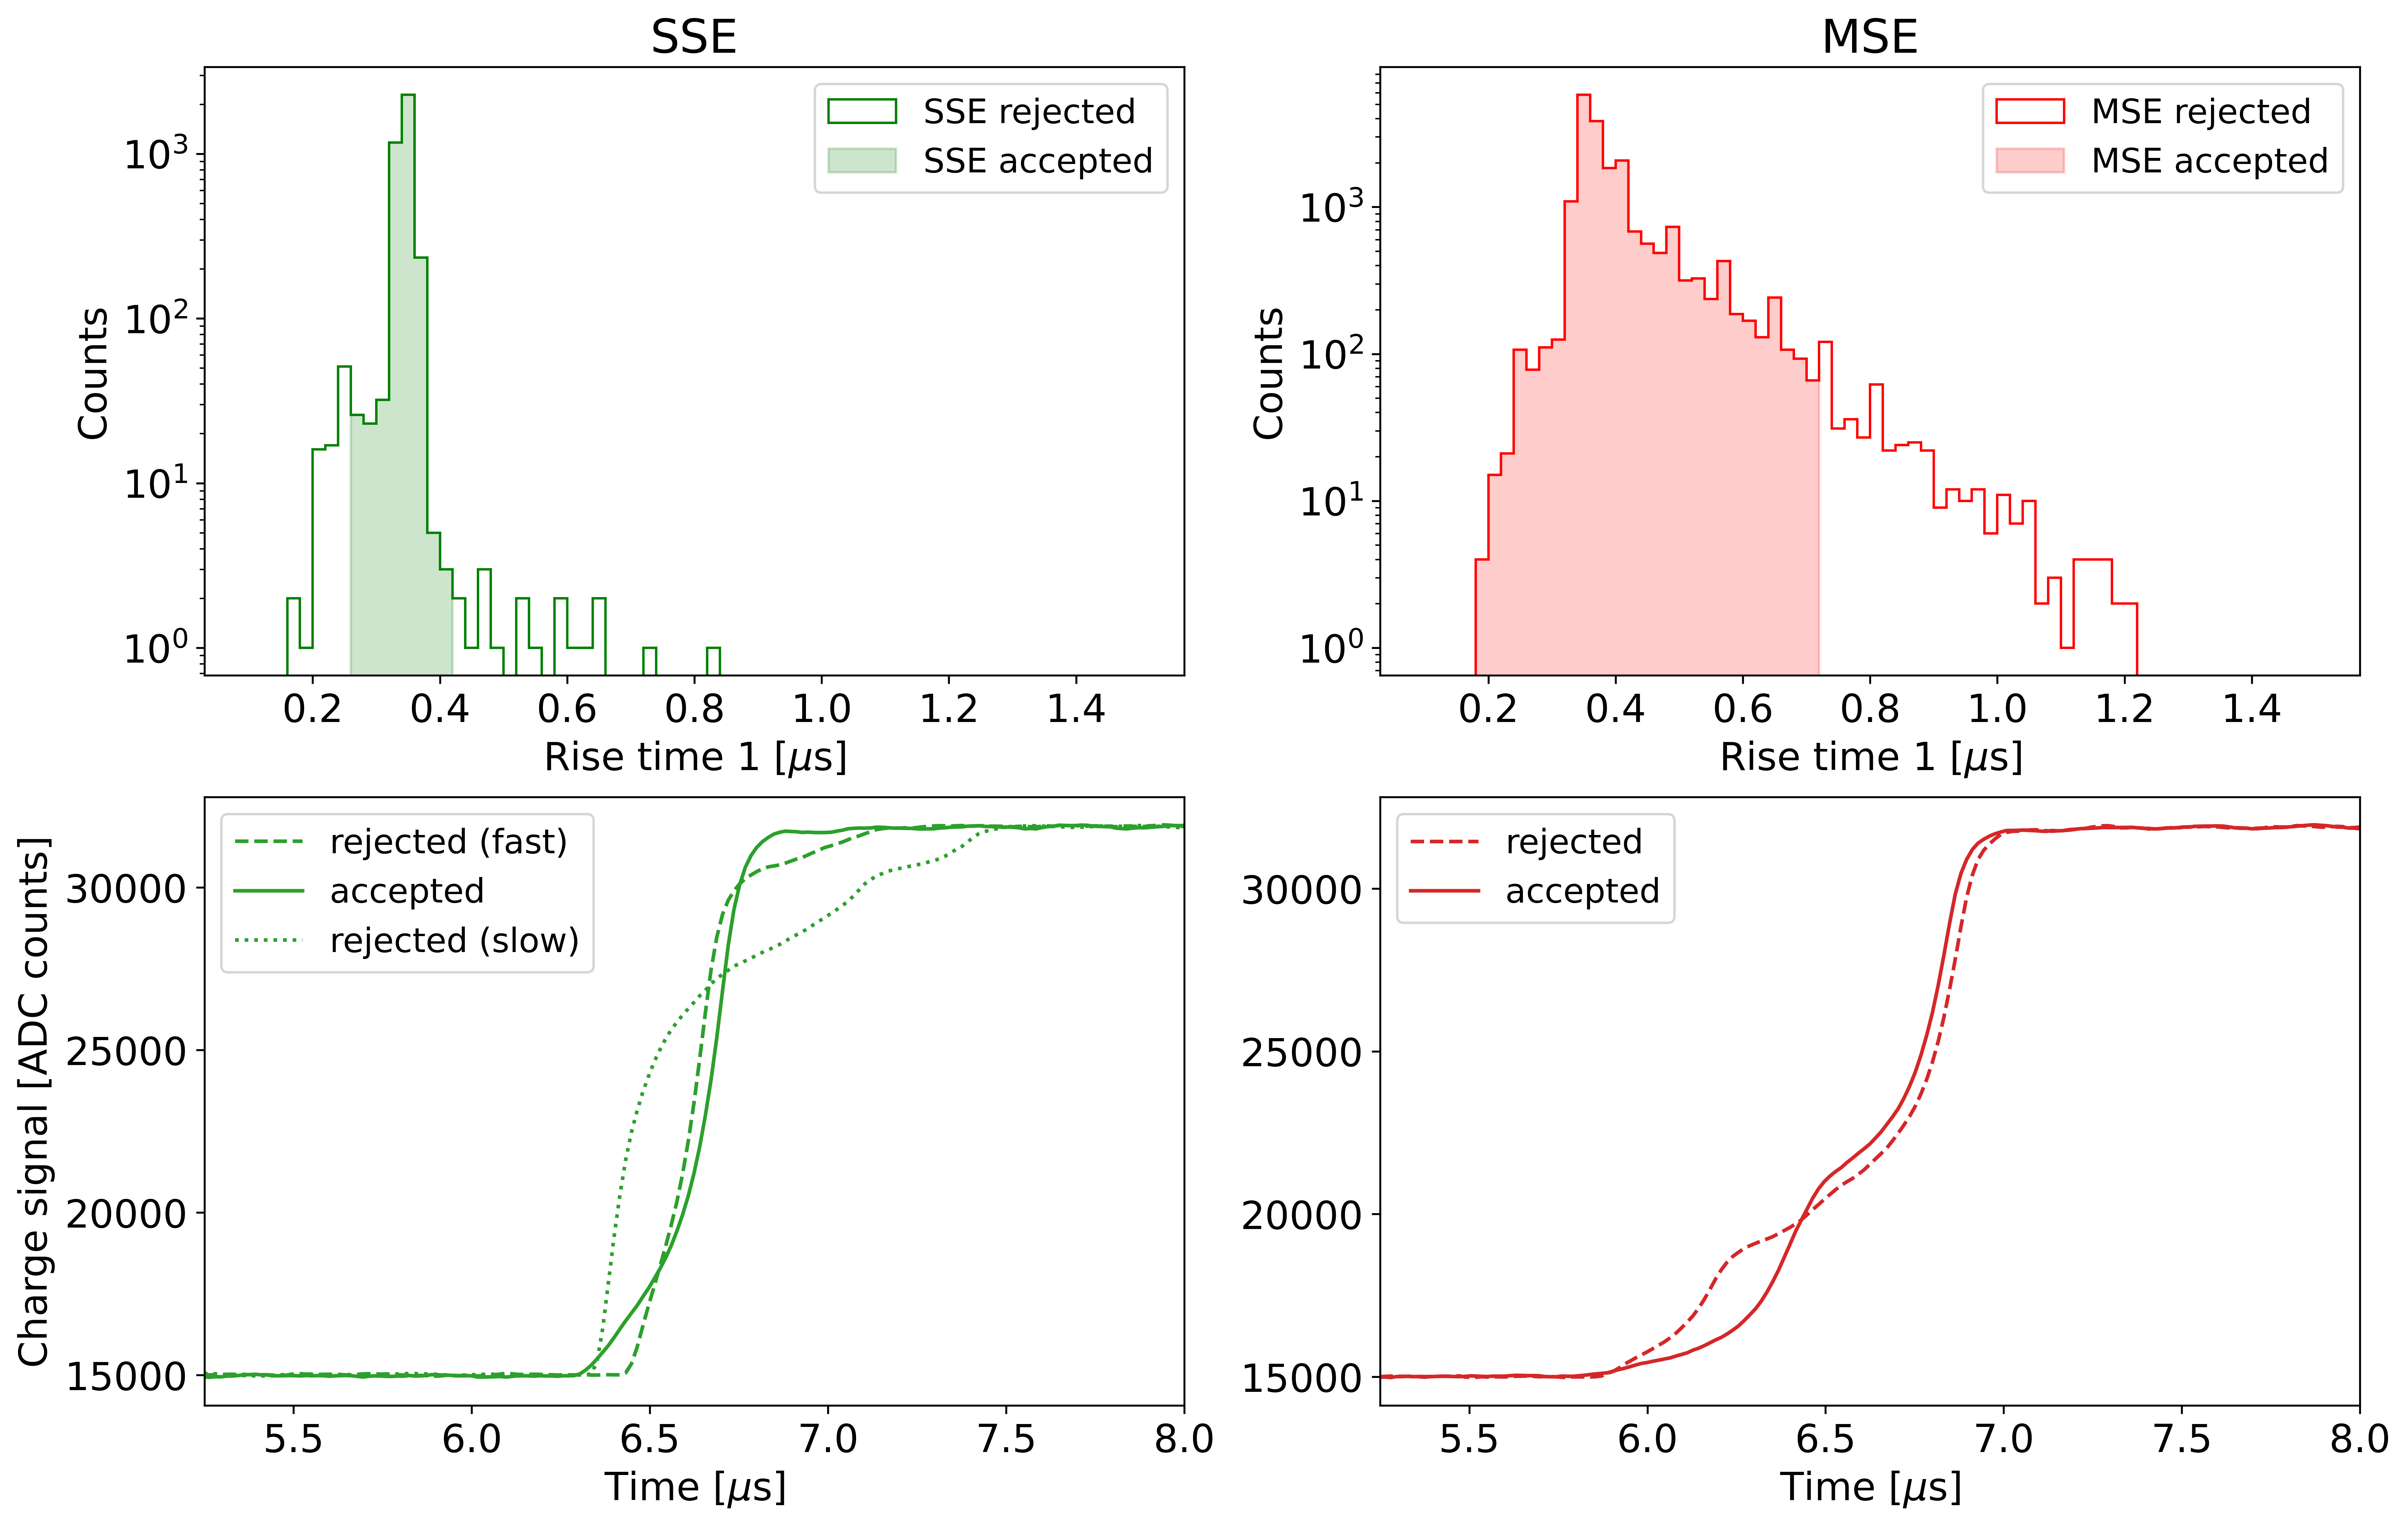
\includegraphics[width=\linewidth]{figures/05_PSD/Plot_DataCleaning_rt1_V02160A.png}
    \caption{Rise time outlier removal ($3 \, \sigma$) for ICPC detector V02160A during period 3. The top panels show histograms of accepted and rejected events; the bottom panels show example waveforms. Single-site events (left) are more homogeneous than multi-site events (right). In the bottom left, an accepted waveform (solid) is compared to outliers with too fast (dashed) and too slow (dotted) rise times. Similar rejection is applied to long-rise-time MSE events (bottom right).}
    \label{fig:datacleaning_rt1}
\end{figure}

For the other quantities described in table~\ref{tab:Data_cleaning_param}, a symmetric $ \pm 2 \, \sigma$ window is applied for outlier rejection. In total, around 8\% of events are rejected in this step. Outlier removal is illustrated in figure~\ref{fig:datacleaning_rt1}, which shows rise time cleaning cuts for single-site and multi-site events, and in figure~\ref{fig:datacleaning_fwhm}, which shows cuts on the FWHM of the peak with the highest amplitude. Both figures include example waveforms of accepted and rejected events. 



\begin{figure}
    \centering
    \includegraphics[width=\linewidth]{figures/05_PSD/Plot_DataCleaning_fwhm_V02160A.png}
    \caption{Peak width outlier removal ($2 \, \sigma$) for ICPC detector V02160A during period 3. The top panels show histograms of accepted and rejected events; the bottom panels show example differentiated waveforms. For multi-site events, only a lower peak width bound is applied to avoid rejecting merged peaks. Bottom left: accepted SSE waveform (solid) vs. rejected broadened peak (dashed). Bottom right: rejected waveform (dashed) with a sharp rise, indicating interaction near the p$^{+}$ electrode.}
    \label{fig:datacleaning_fwhm}
\end{figure}

\subsection{Model training and evaluation}

The Transformer model architecture used in this work is described in section~\ref{sec:04_transformer_used}. It was trained on several datasets, each prepared according to the procedures outlined in the previous subsections. An overview of all datasets used for training is provided in table~\ref{tab:Datasets_overview}. 
The models are trained using four NVIDIA V100 GPUs on the Perlmutter supercomputer at the National Energy Research Scientific Computing Center (NERSC) in Berkeley, California. 
The datasets were split into three parts: 60\% for training (used to optimize model weights), 10\% for validation (used to monitor generalization performance and prevent overfitting), and 30\% for testing. The validation set allows for early stopping, terminating training when the validation loss is no longer improving, and performance monitoring without influencing the model's parameters. 
Since its purpose is monitoring, a relatively small share is sufficient. The test set is strictly held out and used only to report the final model performance; it must be large enough to provide statistically meaningful results without excessively reducing the training data. 
We used a batch size of 512 per GPU, resulting in an effective batch size of 2048.
The loss function used in this work is the combined loss shown in equation~\refeq{eq:combined_loss}. It is optimized using ADAM, described at the end of section~\ref{sec:03_optimization_algorithms}.  

The different models are then evaluated and assessed with several metrics. 
The precision score, defined in equation~\refeq{eq:precision_score}, measures the proportion of correctly identified positive instances among all instances classified as positive. In the context of single-site events, it quantifies the fraction of events classified as SSE that are truly single-site. A high precision score indicates a low number of false positives.

\begin{equation}
\label{eq:precision_score}
	\mathrm{Precision} = \frac{\mathrm{True \; Positive}}{\mathrm{True \; Positive + False \; Positive}} \,. 
\end{equation}

Sensitivity addresses the complementary aspect by quantifying the proportion of true SSE events that are correctly identified. A high sensitivity indicates a low number of false negatives, meaning the model effectively captures most of the true positive cases: 

\begin{equation}
\label{eq:sensitivity_score}
	\mathrm{Sensitivity} = \frac{\mathrm{True \; Positive}}{\mathrm{True \; Positive + False \; Negative}} \,.
\end{equation}

In machine learning, the F1-score is commonly reported alongside precision and sensitivity as a measure of the balance between the two:

\begin{equation}
\label{eq:f1_score}
	\mathrm{F_1} = 2 \; \frac{\mathrm{Precision} \cdot \mathrm{Sensitivity}}{\mathrm{Sensitivity + Precision}} \,.
\end{equation}


A confusion matrix provides a compact graphical representation of classification performance. For $n_{\mathrm{label}}$ classes, it is an $n_{\mathrm{label}} \times n_{\mathrm{label}}$ matrix in which each row corresponds to the ground truth and each column to the model's predicted class. The diagonal entries indicate correct classifications, while the off-diagonal entries represent misclassifications, including false positives and false negatives~\cite{murphy_probabilistic_2022}.  

\begin{table}
\centering
\caption{Datasets used for training the Transformer, only including ICPC detector waveforms. The data size indicates the total number of waveforms in the dataset. In the second Transformer model, $p^{+}$ and $n^{+}$ events are combined into a single surface label.}
\begin{tabular}{||c | c | c | c | c||} 
 \hline
 \textbf{Transformer} & \textbf{Periods} & \textbf{Data size} & \textbf{Isotopes} & \textbf{Labels} \\ 
 \hline
 Model 1 & 3 - 10 & 12.5 $\times 10^6$ & $^{228}$Th & SS, MS, p$^{+}$, n$^{+}$ \\ 
 \hline
 Model 2 & 3 - 11 & 14.0 $\times 10^6$ & $^{228}$Th, $^{56}$Co & SS, MS, surface \\
 \hline
 Model 3 & 3 \& 11 & 3.0 $\times 10^6$ & $^{228}$Th, $^{56}$Co & SS, MS, p$^{+}$, n$^{+}$ \\
 \hline
\end{tabular}
\label{tab:Datasets_overview}
\end{table}


\subsubsection{First Transformer model}

The first model configuration was trained on 12.5 million waveforms extracted from the energy ranges of the four dominant $^{228}$Th calibration peaks. These include the double-escape peak of $^{208}$Tl at 1592.5 keV, the full-energy peak of $^{212}$Bi at 1620.5 keV, and the single-escape and full-energy peaks of $^{208}$Tl at 2103.5 keV and 2614.5 keV, respectively. 
We used waveforms from periods 3 to 10 for this dataset. 

The true labels were assigned according to the classification scheme outlined in table~\ref{tab:event_classification}. The classification performance is illustrated by the confusion matrix in figure~\ref{fig:Confusionmatrix_icpc_v1}, which shows the precision. The corresponding scores are summarized in table~\ref{tab:Scores_icpc_v1}. The model achieves very high precision for both single-site and multi-site events, as well as strong precision for surface event classification. Sensitivity is notably lower for SSE and p$^+$ events in contrast to MSE and n$^+$ events, indicating some degree of cross-contamination between these classes. Despite this, all F1-scores exceed 95\%, demonstrating an overall excellent classification performance.

\begin{figure}
    \centering
    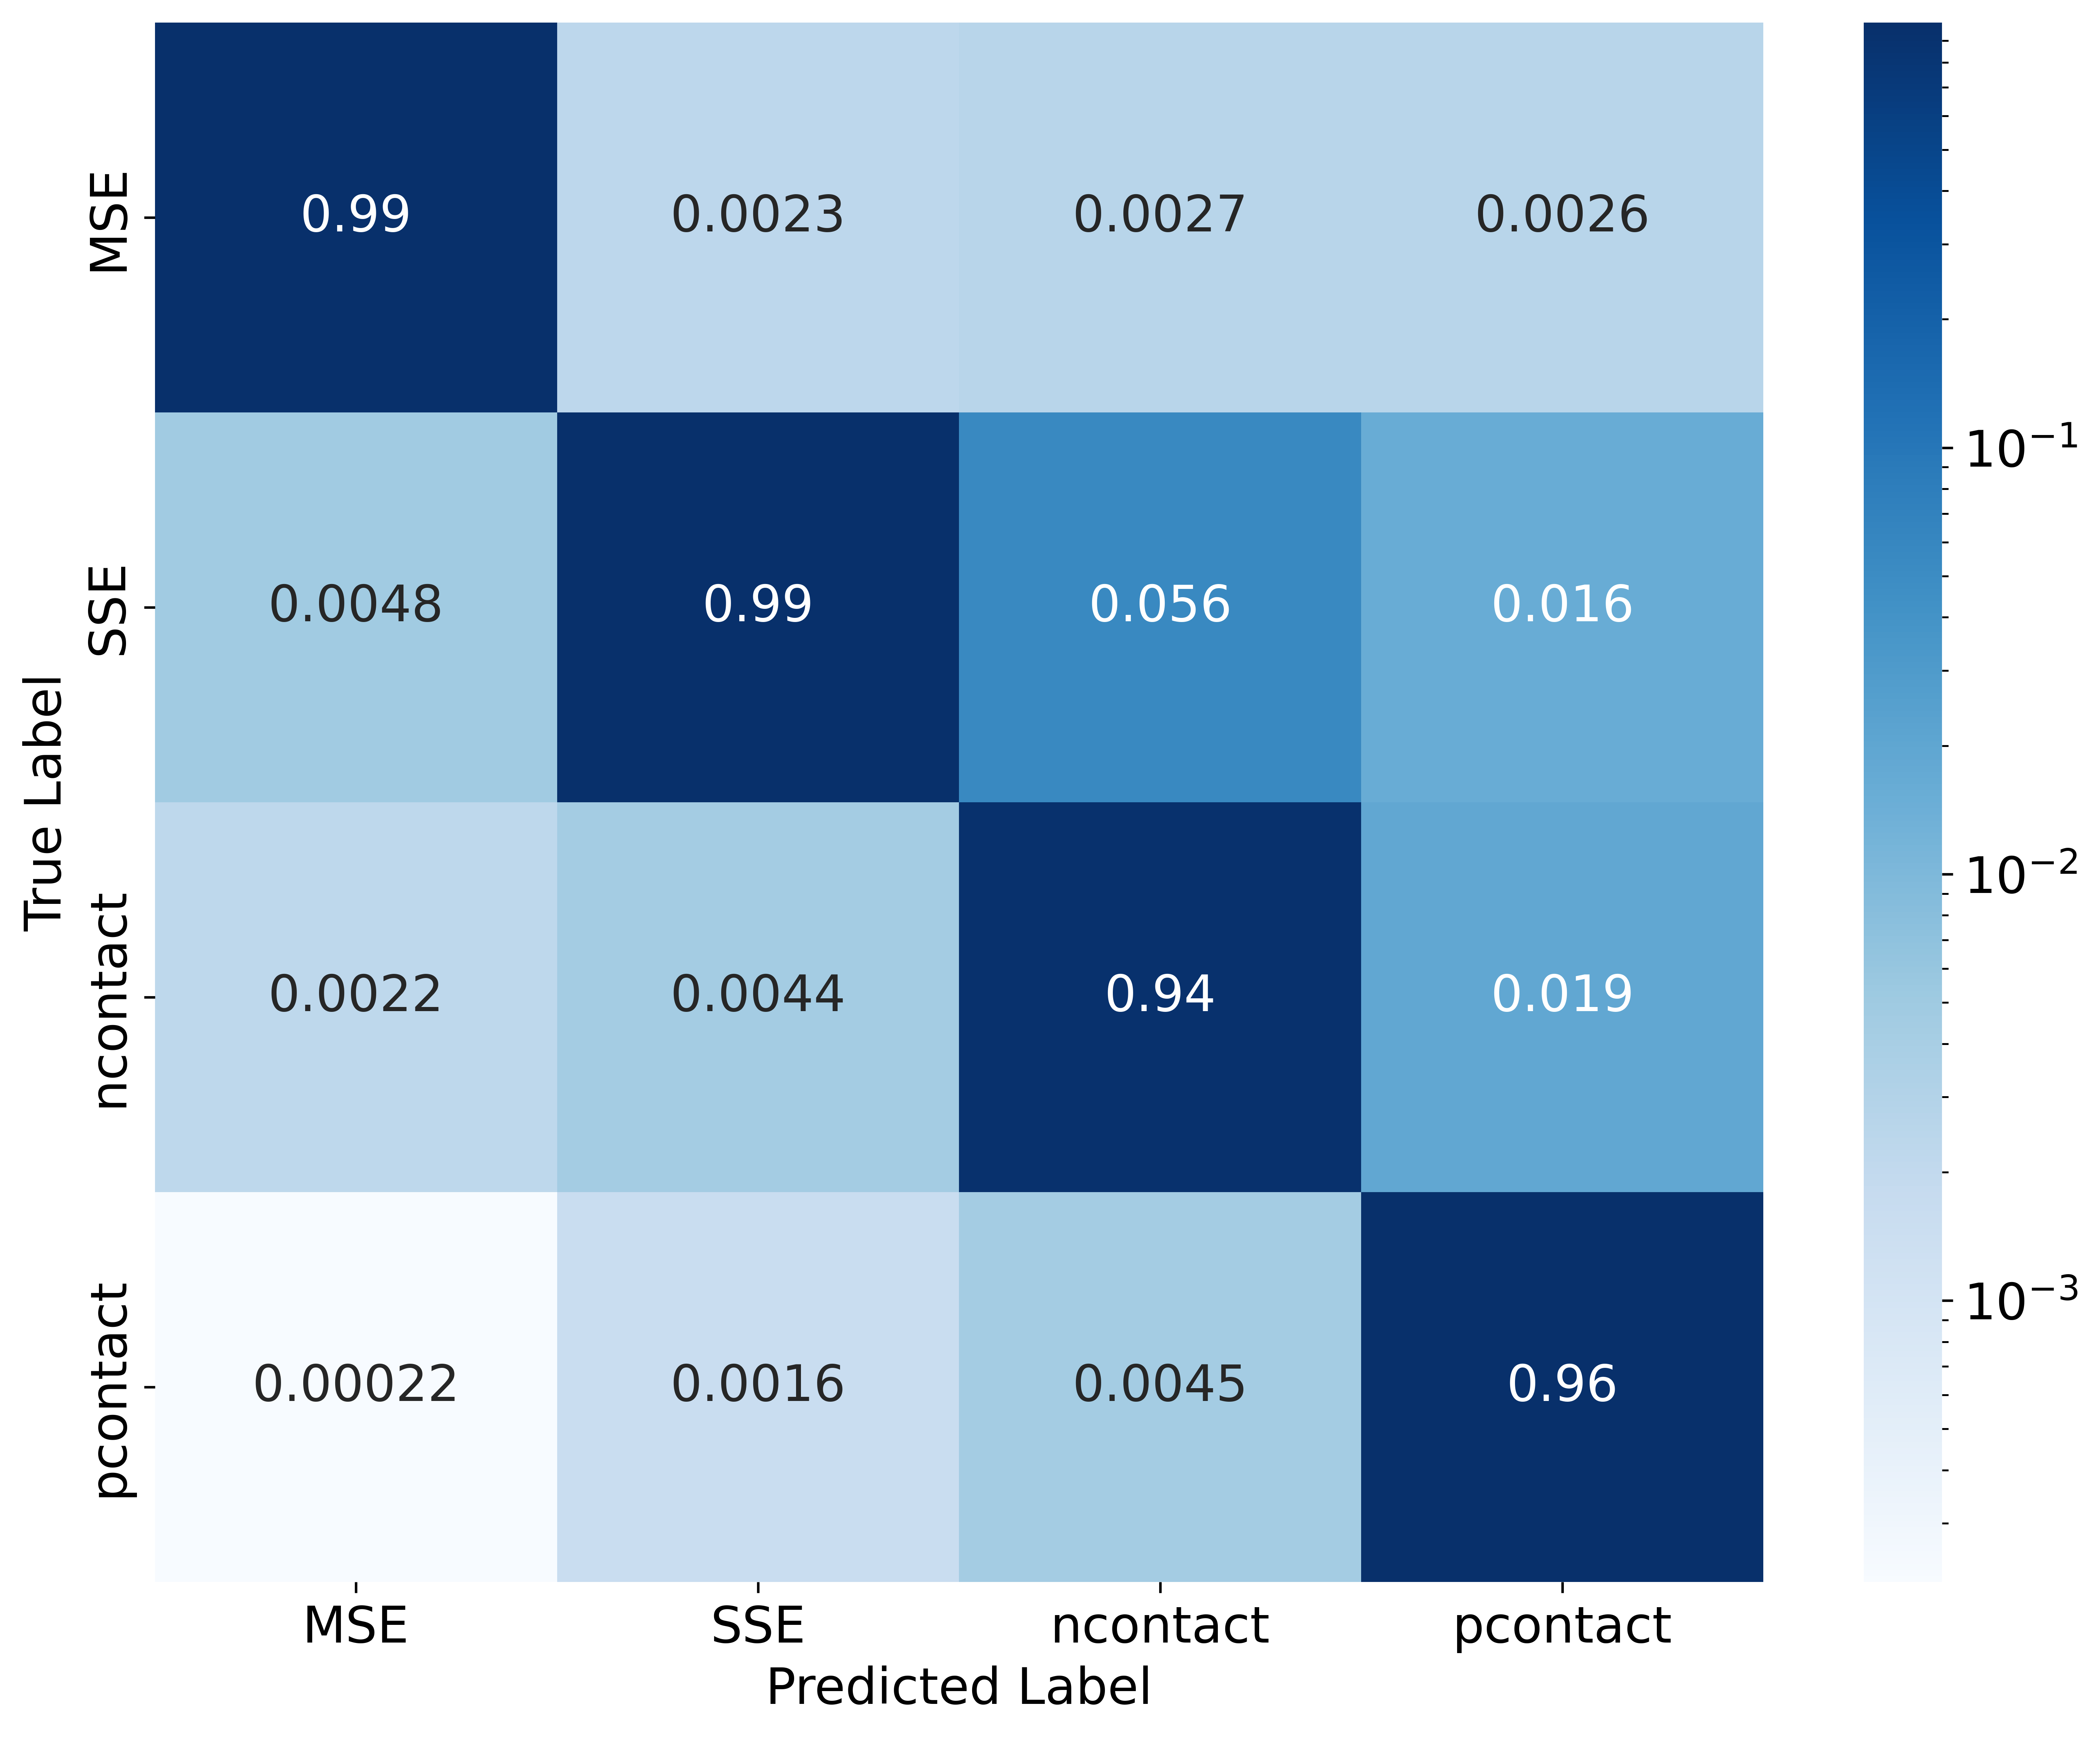
\includegraphics[width=0.75\linewidth]{figures/05_PSD/Results_confusionmatrix_icpc_v1.png}
    \caption{Confusion matrix of model one, with precision scores shown on the diagonal. The model was trained on 12.5 million $^{228}$Th calibration waveforms. Multi-site and single-site events are classified with high precision ($>99\%$), while both surface event types show some misclassification but still achieve precision scores above 90\%.} 
\label{fig:Confusionmatrix_icpc_v1}
\end{figure}

\begin{table}
\centering
\caption{Classification scores for the first Transformer model. Precision is the fraction of correct positive predictions, while sensitivity refers to the fraction of true positives correctly identified. The F1-score combines both.}
\begin{tabular}{||c | c | c | c | c||} 
 \hline
 \textbf{Class} & \textbf{Precision} & \textbf{Sensitivity} & \textbf{F1-score} & \textbf{Support} [$\times 10^6$] \\ 
 \hline
 SSE & 0.992 & 0.925 & 0.957 & 1.03 \\
 \hline
 MSE & 0.993 & 0.996 & 0.994 & 1.47 \\
  \hline
 n$^+$ & 0.937 & 0.992 & 0.964 & 1.15 \\
 \hline
 p$^+$ & 0.963 & 0.937 & 0.950 & 0.12 \\
 \hline
 Weighted avg	&  0.975 & 0.974 & 0.974 & 3.76  \\ 
 \hline
\end{tabular}
\label{tab:Scores_icpc_v1}
\end{table}


\subsubsection{Second Transformer model} 

For the second model, the training data was extended. In addition to the four primary $^{228}$Th calibration peaks, we included seven additional energy peaks from a dedicated $^{56}$Co calibration run, all of which are DEPs: 1012.8~keV, 1576.5~keV, 1987.6~keV, 2180.0~keV, 2231.5~keV, 2251.1~keV, and 2429.2~keV. 

Using additional energy regions should improve the model's flexibility.
Furthermore, the two surface event classes (n$^+$ and p$^+$) were merged into a single surface label. Apart from these changes, the second model is architecturally identical to the first.

This resulted in a total of 11 distinct energy regions, used to extract 14 million waveforms for training. The resulting model demonstrates classification precision across all event types ($98\%$), shown in the confusion matrix in figure~\ref{fig:Confusionmatrix_icpc_v2}, and the summary table~\ref{tab:Scores_icpc_v2}. Furthermore, the model achieves exceptionally high sensitivity across all classes, all with F1-scores exceeding 98\%. While such uniformly high scores indicated excellent classification performance, it's important to check that this isn't due to overfitting. 

\begin{figure}[t]
    \centering
    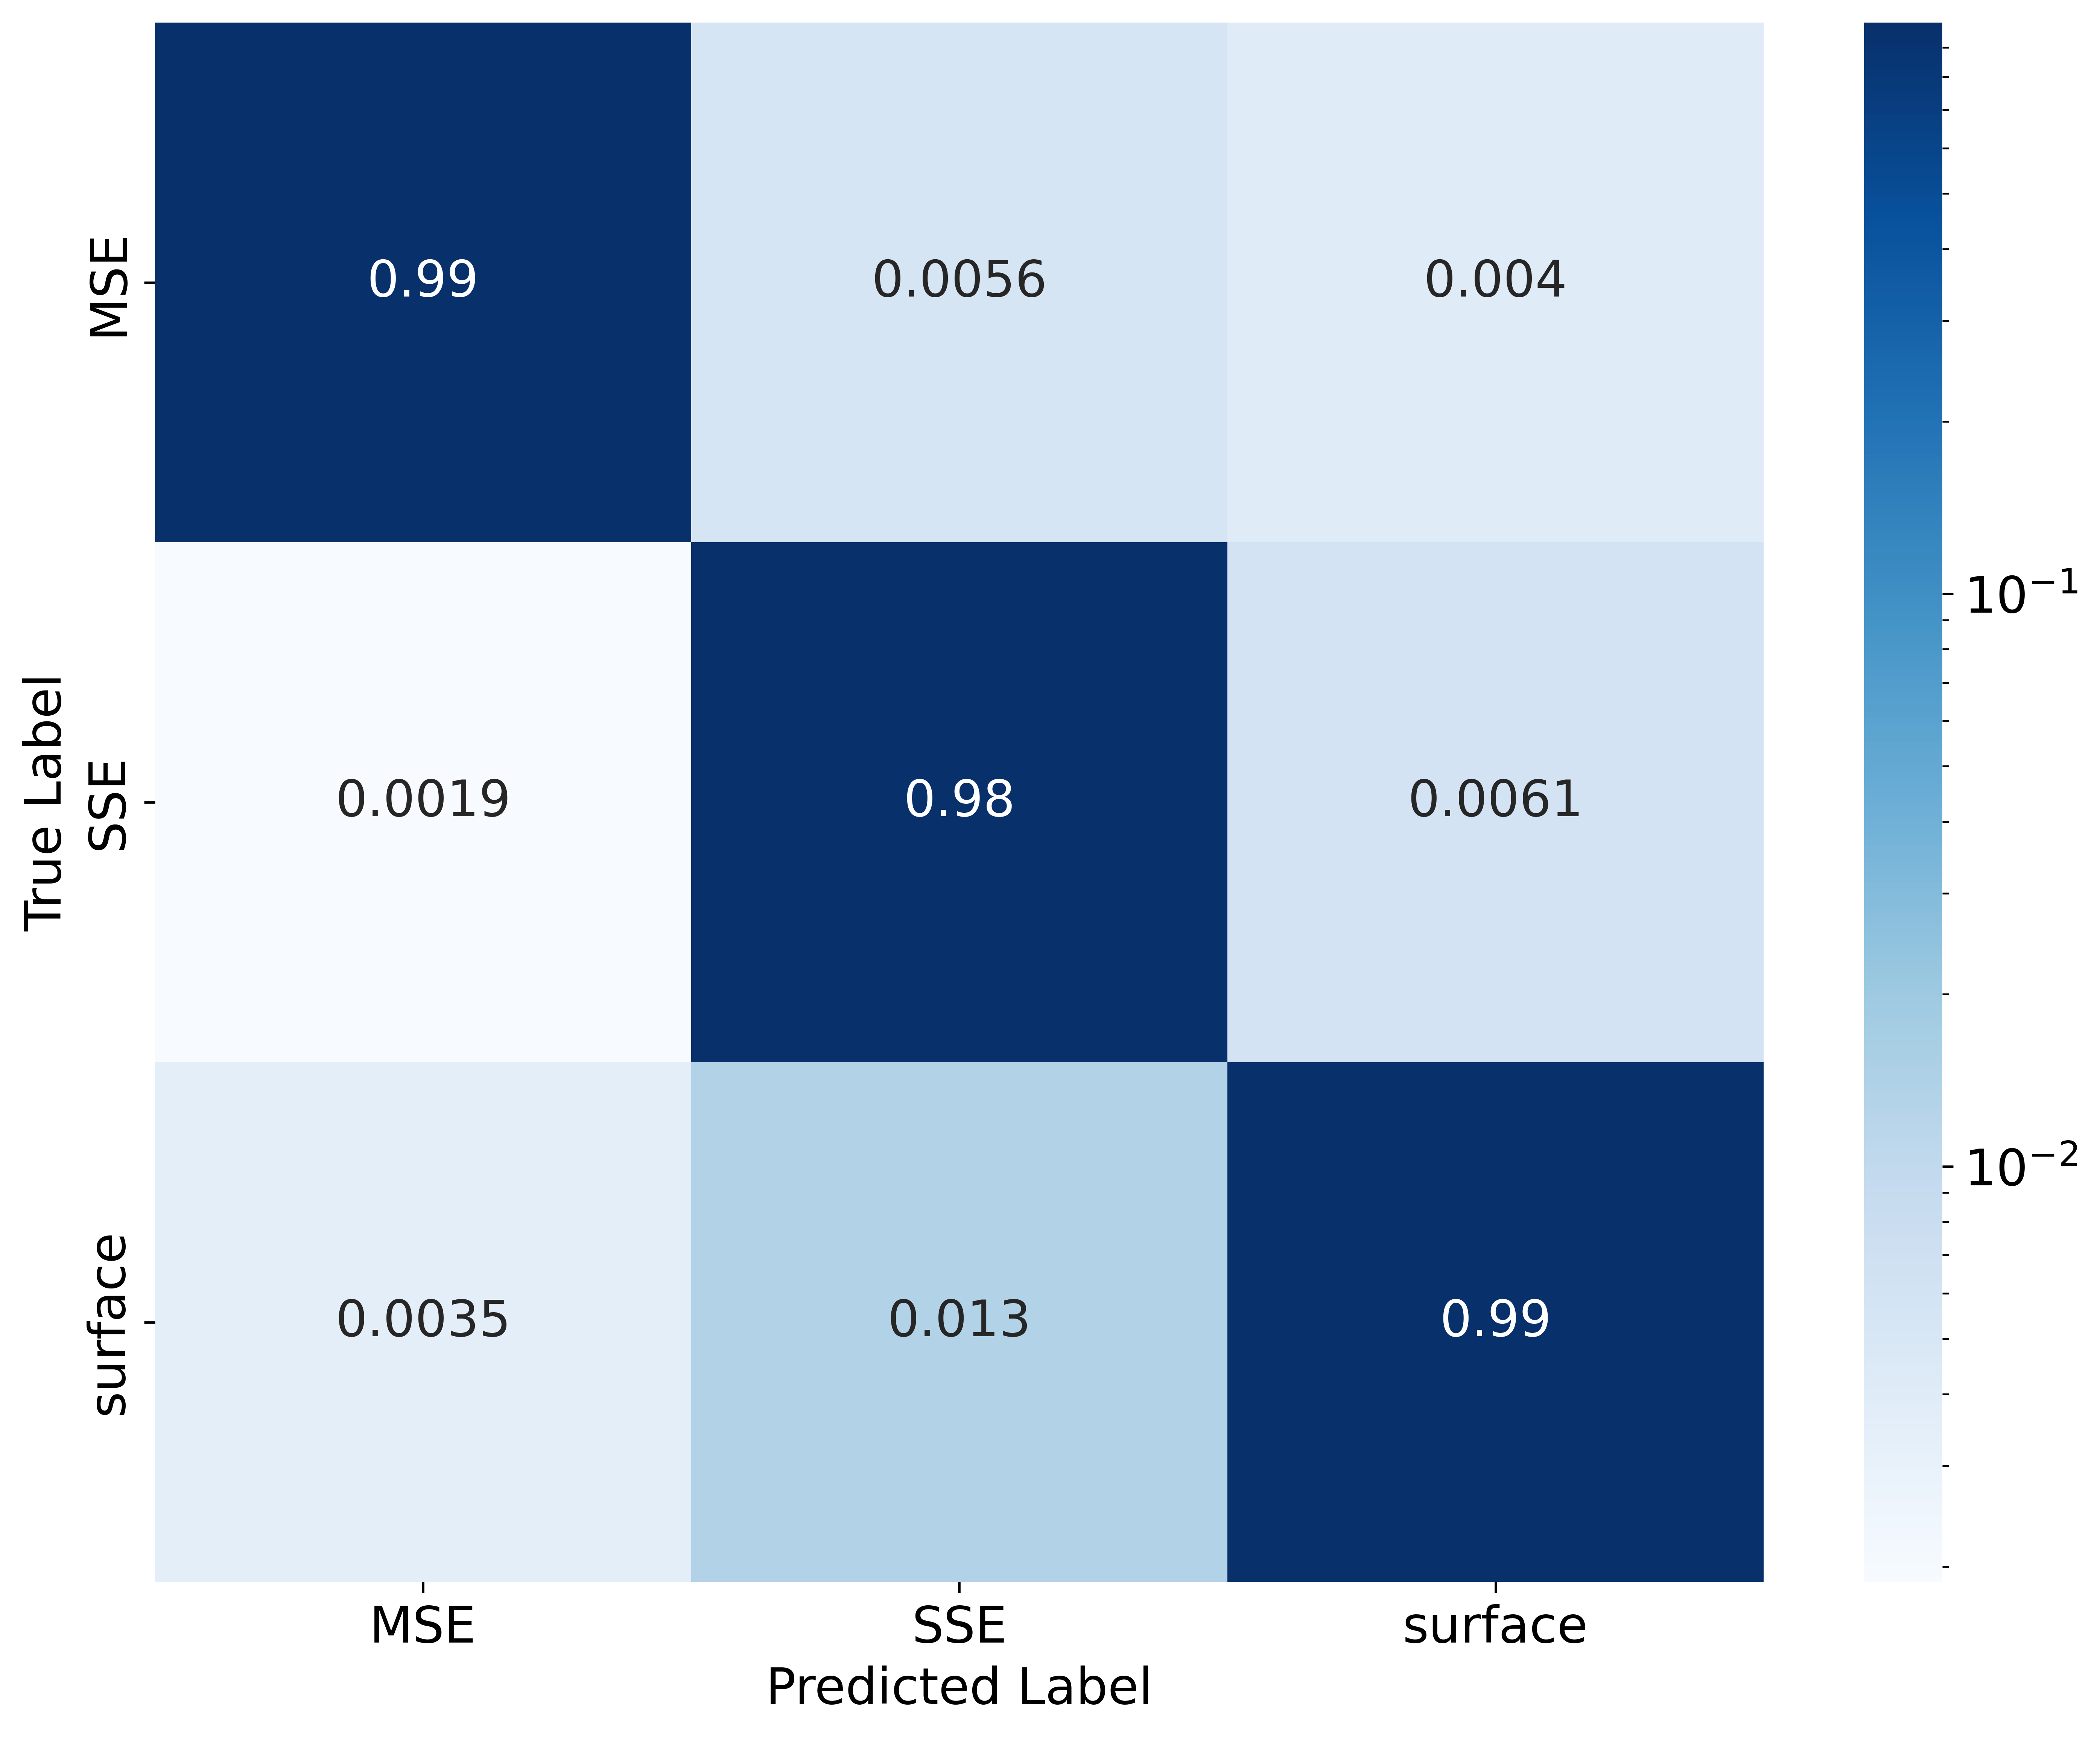
\includegraphics[width=0.75\linewidth]{figures/05_PSD/Results_confusionmatrix_icpc_v2.png}
    \caption{Confusion matrix of model two, where we trained on 14.0 million events. This testing includes 3.3 million events. All event categories are classified with high precision, each exceeding 98\%.} 
\label{fig:Confusionmatrix_icpc_v2}
\end{figure}


\begin{table}
\centering
\caption{Classification scores for the second Transformer model: Precision and sensitivity exceed 98\% for all classes.}
\begin{tabular}{||c | c | c | c | c||} 
 \hline
 \textbf{Class} & \textbf{Precision} & \textbf{Sensitivity} & \textbf{F1-score} & \textbf{Support} [$\times 10^6$] \\ 
 \hline
 SSE & 0.981 & 0.989 & 0.985 & 0.61 \\
 \hline
 MSE & 0.995 & 0.993 & 0.994 & 0.40 \\
  \hline
 surface & 0.990 & 0.986 & 0.988 & 0.55 \\
 \hline
 Weighted avg & 0.989 & 0.989 & 0.989 & 1.56 \\ 
 \hline
\end{tabular}
\label{tab:Scores_icpc_v2}
\end{table}



\subsubsection{Third Transformer model}

A third model was also prepared using a new dataset based on $^{228}$Th and $^{56}$Co calibration data. While it covered the same energy regions as the second model, we wanted to maintain the balance between the two different calibrations. Therefore, we selected only a single $^{228}$Th calibration period (period 3). In addition, the surface-event labels were separated again into distinct p$^+$ and n$^+$ categories. 
However, this model performed poorly: it failed to generalize beyond the training data and exhibited inconsistent classification across detectors. Due to these issues, the model was deemed unsuitable for further evaluation and was excluded from the analysis. The exact cause of the poor performance remains unclear, but it may be related to the label noise in the $^{56}$Co dataset. 


\subsubsection{Network comparison and performance on \texorpdfstring{$2 \nu \beta \beta$ decay events}{}}

The classification scores of the three Transformer models were evaluated on a test dataset consisting of calibration events at well-defined $\gamma$-ray energy peaks. For the PSD cut to be applicable in LEGEND-200, the models must generalize beyond these narrow energy regions, in particular to the vicinity of $Q_{\beta \beta} = 2039$~keV. Reliable single-site classification at lower energies is important, as it enables validation of PSD efficiency using the continuous $2 \nu \beta \beta$ decay spectrum present in physics data. In particular, the energy range between 1000 and 1300~keV, used in this analysis to extract the PSD efficiency at $Q_{\beta \beta}$, is a key validation region. Figure~\ref{fig:SSE_cuts_2vbb} shows that, for $E < 1$~MeV, only model 1 maintains a stable SSE efficiency across the spectrum, whereas the other models exhibit inconsistent behavior.  



\begin{figure}[t]
    \centering
    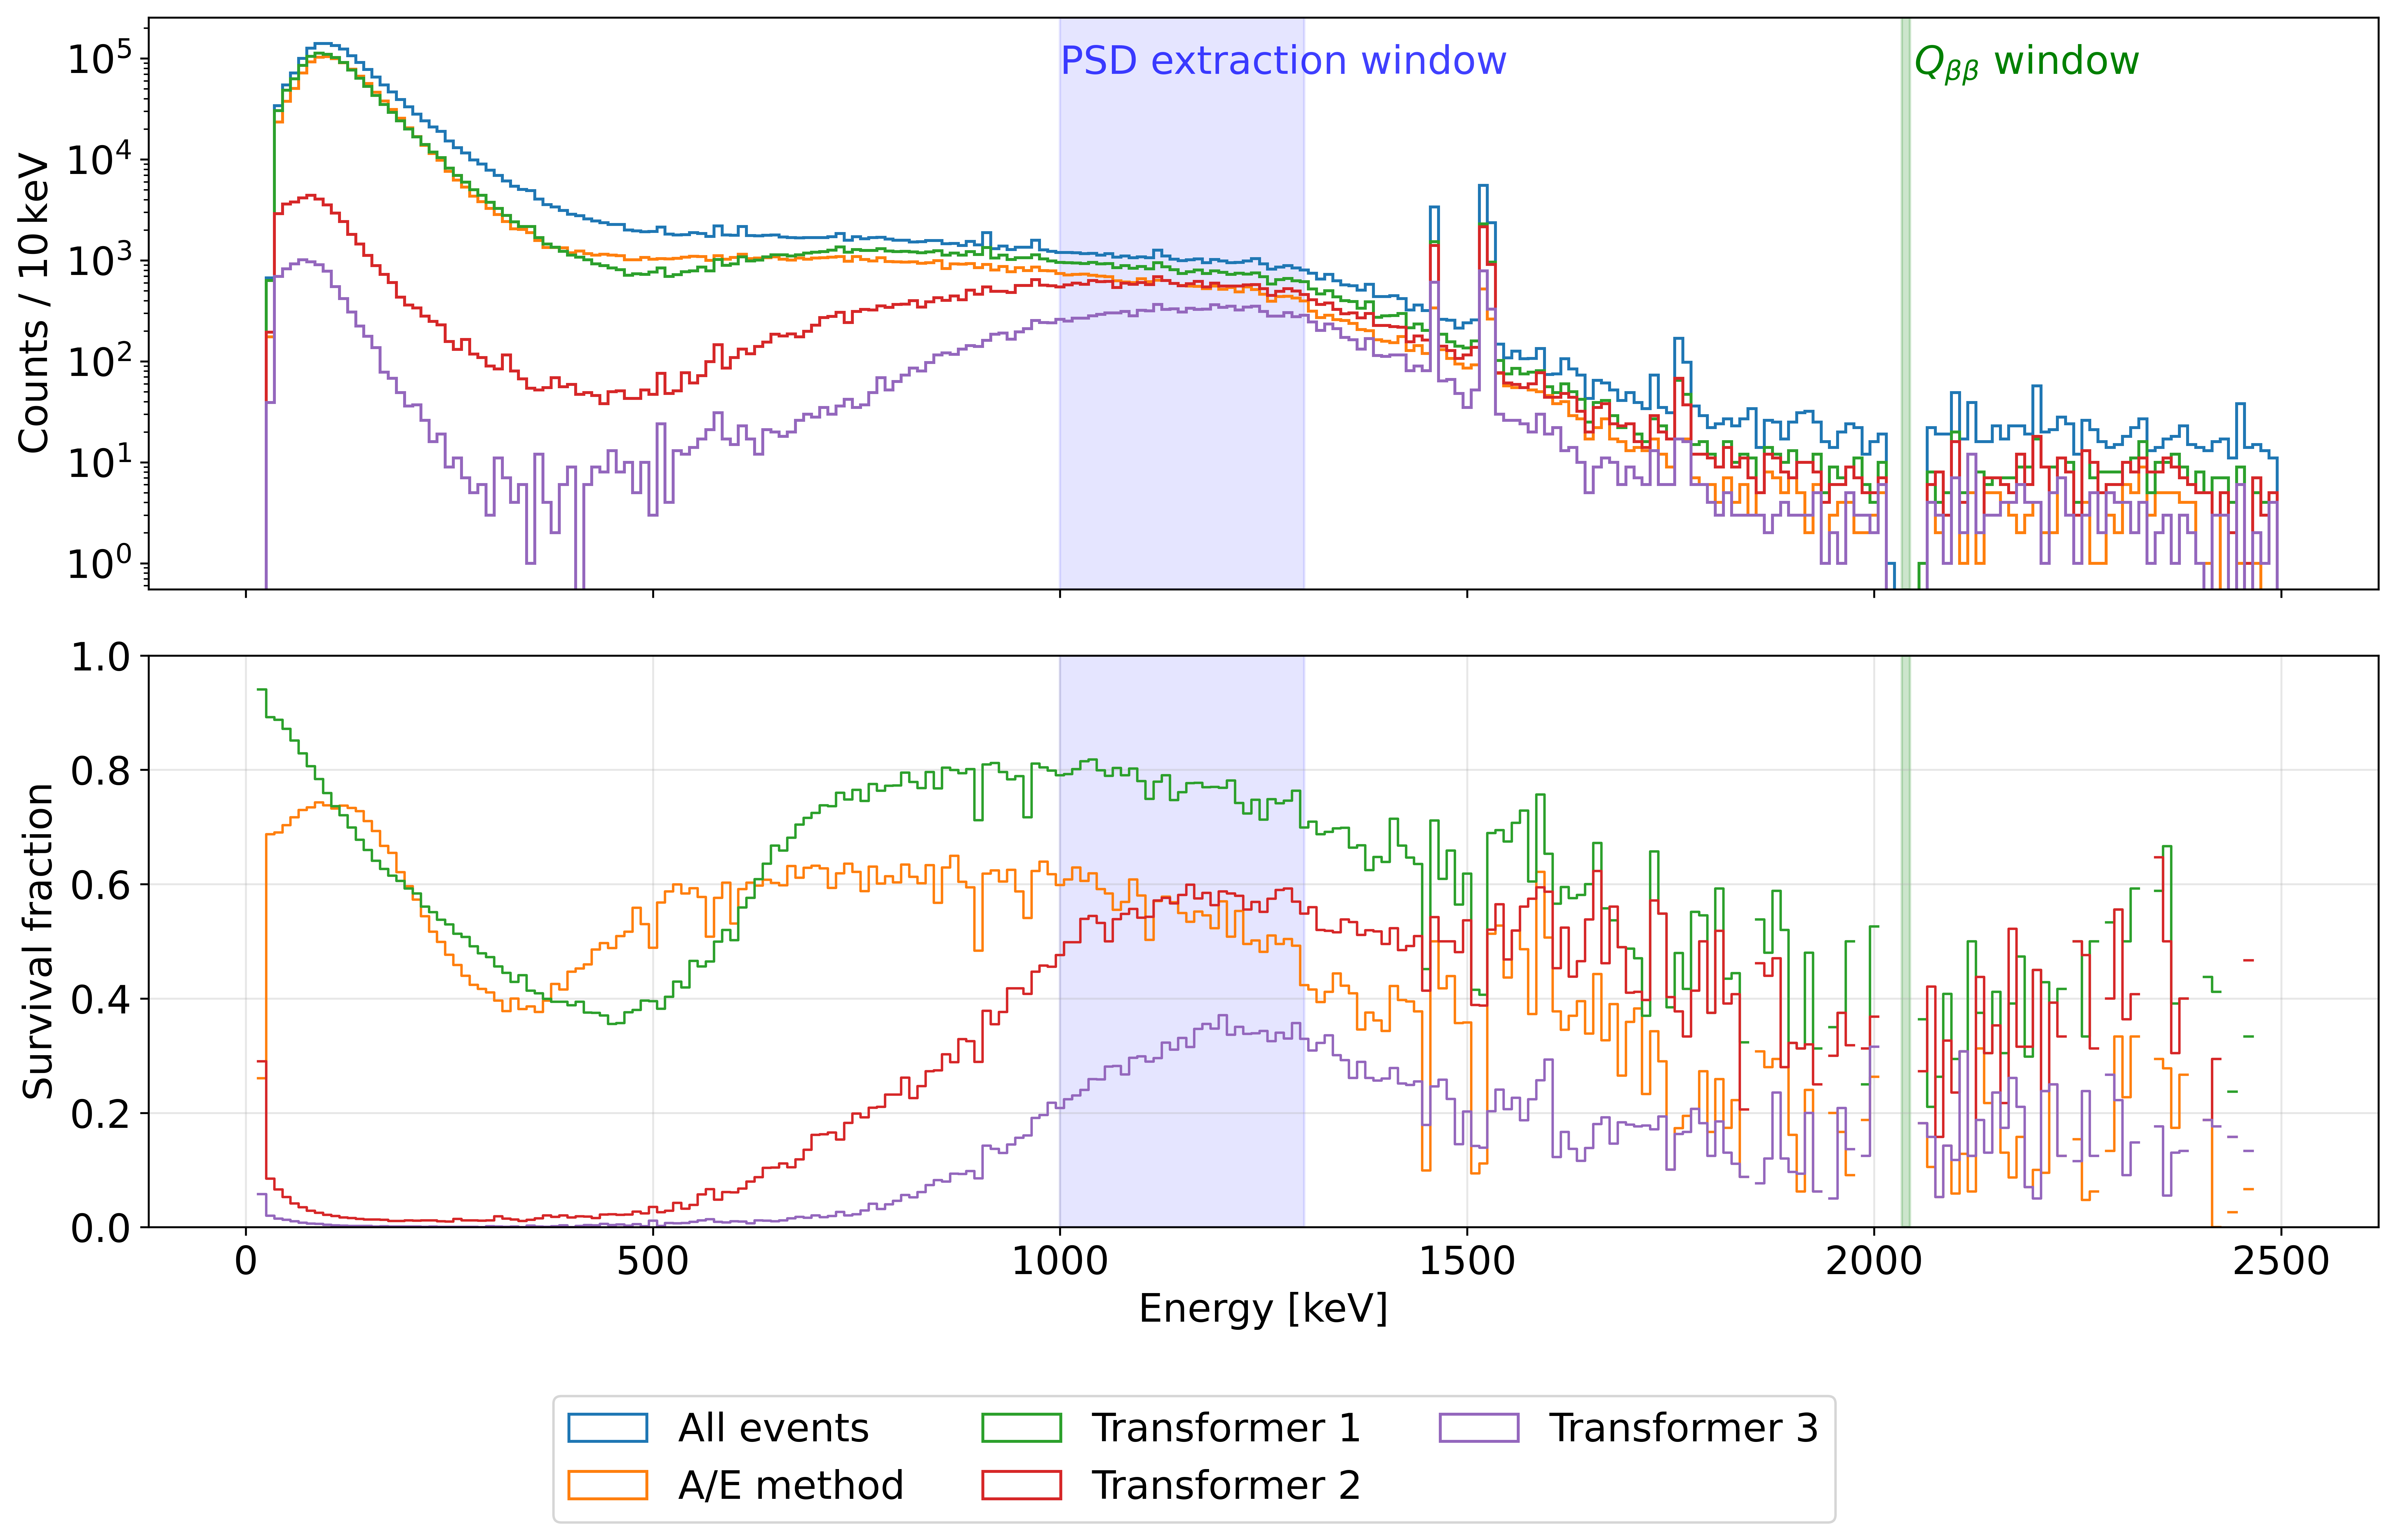
\includegraphics[width=\linewidth]{figures/05_PSD/SSE_cuts_2vbb.png}
    \caption{Energy spectra of the $2 \nu \beta \beta$ decay population, with different PSD cuts, applied (top), and the corresponding survival fractions (bottom). The spectra include all physics runs listed in section~\ref{sec:04_LEGEND_data}, corresponding to a total exposure of $40.3\, \mathrm{kg} \cdot \mathrm{yr}$. We see that Transformer models 2 and 3 generalize very poorly for the low-energy part of the spectrum, while the A/E cut generally works better at very low energies. }
\label{fig:SSE_cuts_2vbb}
\end{figure}



\subsection{Pulse shape discrimination efficiency at \texorpdfstring{$Q_{\beta \beta}$}{}}
To evaluate the effect of PSD efficiencies on the expected $0 \nu \beta \beta$ decay half-life, the PSD efficiency at $Q_{\beta \beta}$, denoted as $\epsilon_{\mathrm{PSD}}$, must be determined. We adopt a similar procedure as developed by the LEGEND-200 collaboration, described in~\cite{lnote_24013}. 
In this analysis, only Mirion ICPC detectors are considered, which allows for consistent PSD cut definitions throughout the full analysis. Furthermore, the LEGEND-200 collaboration has decided to focus on ICPC detectors. Since we have no pure SSE populations at $Q_{\beta \beta}$ to estimate the efficiencies, we assume a linear energy dependence and extrapolate the efficiency at $Q_{\beta \beta}$. 

We therefore calculate the PSD efficiency as:

\begin{equation}
\label{eq:psd_eff_qbb}
    \epsilon_{\mathrm{PSD}} = \tilde{\epsilon}_{\mathrm{PSD}} + \langle \delta_{\mathrm{run}} \rangle + \epsilon_{2 \nu \beta \beta} \,,
\end{equation}

\noindent where $\tilde{\epsilon}_{\mathrm{PSD}}$ denotes the uncorrected PSD efficiency at $Q_{\beta \beta}$. The correction term $\langle \delta_{\mathrm{run}} \rangle$ accounts for time-dependent variations in the PSD performance during data taking, and $\epsilon_{2 \nu \beta \beta}$, compensates for differences in the single-site event population between $2 \nu \beta \beta$ decays and the double escape peak calibration data. 
The energy dependence of SSE detection efficiency using the A/E parameters arises from three main physical effects \cite{comellato_topologies_2023}: 

\begin{enumerate}
    \item Bremsstrahlung becomes more probable at higher energies, leading to the emission of secondary photons. This can spatially separate the energy deposition and reduce the A/E value, causing SSEs to be misclassified as MSE, thereby lowering the detection efficiency at $Q_{\beta \beta}$ compared to the $^{208}$Tl DEP~\cite{comellato_charge_2021}.
    \item Charge cloud self-repulsion increases with energy due to a higher number of induced charges. This results in longer drift times and broader waveforms, which in turn reduce the signal amplitude and the A/E value. As a result, the detection efficiency at $Q_{\beta \beta}$ is further reduced~\cite{Radford_2012}. 
    \item Electronic noise becomes less relevant at higher energies, which tends to increase the detection efficiency. However, this effect is generally outweighed by the first two.
\end{enumerate}

Together, these effects imply that the PSD efficiency decreases at higher energies. In this work, we estimate the PSD efficiency at three different energy regions. The method for extracting the efficiency in each region is presented in the following subsections:

\begin{itemize}
	\item In the 1000-1300 keV interval, using the $2 \nu \beta \beta$ decay background (PSD extraction window)
	\item At the 1592.5 keV DEP from $^{208}$Tl
	\item At the 2231.5 keV DEP from $^{56}$Co.
\end{itemize}


\subsubsection{PSD efficiency for \texorpdfstring{$2 \nu \beta \beta$}{} decay events}

To estimate the PSD efficiency for $2 \nu \beta \beta$ decay events, the Transformer models were tested on all periods listed in table~\ref{tab:periods_runs} for a total exposure of $40.3\, \mathrm{kg} \cdot \mathrm{yr}$. The PSD efficiency can be evaluated at different energy regions within the spectrum. For this analysis, we use the 1000-1300 keV window because this region offers high statistics and is relatively free from prominent gamma lines.
An alternative energy range between 1525 and 1750 keV could be used if contributions from gamma lines are subtracted. However, this region suffers from significantly lower event statistics. Therefore, we rely exclusively on the lower-energy window for the PSD efficiency extraction. It is estimated as follows:

\begin{equation}
\label{eq:eff_2vbb}
    \epsilon_{2 \nu \beta \beta} = \frac{\frac{T_p}{T_p + T_f} - \lambda_B \lambda_{Bp}}{1 - \lambda_B} \,.
\end{equation}

\noindent Here, $T_p$ and $T_f$ denote the number of events that pass or fail the PSD cuts, respectively. 
The parameter $\lambda_B$ represents the fraction of events in the window that originate from the background, and $\lambda_{Bp}$ is the fraction of those background events that pass the cuts. 

The value of $\lambda_{B}$ is derived from the expected number of $2 \nu \beta \beta$ decays based on exposure, detection efficiency, and the known half-life. A detailed background analysis for LEGEND-200 by Calgaro et al. determined $\lambda_B = (8.7 \pm 1.7) \%$, which we adopt in this analysis~\cite{lnote_24007}. 

Assuming the background events are equally likely to pass or fail the PSD cut, we set $\lambda_{Bp} = (50 \pm \frac{1}{\sqrt{12}})~\% $, corresponding to a uniform distribution. The uncertainty on $T_p$ and $T_f$ is assumed to follow Poisson statistics.
The uncertainty on $\epsilon_{2 \nu \beta \beta}$ is given by

\begin{align}
\sigma_{\epsilon_{2 \nu \beta \beta}} = \Bigg[ &
\left( \frac{\partial \epsilon}{\partial T_p} \cdot \sigma_{T_p} \right)^2
+ \left( \frac{\partial \epsilon}{\partial T_f} \cdot \sigma_{T_f} \right)^2 \notag \\
& + \left( \frac{\partial \epsilon}{\partial \lambda_B} \cdot \sigma_{\lambda_B} \right)^2
+ \left( \frac{\partial \epsilon}{\partial \lambda_{Bp}} \cdot \sigma_{\lambda_{Bp}} \right)^2
\Bigg]^{1/2} \notag \\
= \Bigg[ &
\left( \frac{\frac{T_f}{(T_p + T_f)^2}}{1 - \lambda_B} \cdot \sigma_{T_p} \right)^2 
+ \left( \frac{\frac{-T_p}{(T_p + T_f)^2}}{1 - \lambda_B} \cdot \sigma_{T_f} \right)^2 \notag \\
& + \left( \frac{\frac{T_p}{T_p + T_f} - \lambda_{Bp}}{(1 - \lambda_B)^2} \cdot \sigma_{\lambda_B} \right)^2
+ \left( \frac{-\lambda_B}{1 - \lambda_B} \cdot \sigma_{\lambda_{Bp}} \right)^2 \Bigg]^{1/2}
\label{eff_2vbb_err} \,.
\end{align}


\subsubsection{PSD efficiency at double escape peaks}

The PSD efficiency at the double escape peaks is determined by fitting the peaks separately for events that pass and events that fail the PSD cut. Example fits are shown in figure~\ref{fig:peakfit_example_Tl} and figure~\ref{fig:peakfit_example_Co} for the $^{208}$Tl and $^{56}$Co DEPs, respectively.  
The full fit function is given by:

\begin{equation}
\label{eq:fit_function_gauss_lin_step}
    f(x, A, \mu, \sigma, a, b, d) = A \cdot e^{\frac{-(x - \mu)^2}{2 \sigma^2}} + \frac{d}{2} \cdot \mathrm{erfc} \left[ \frac{x - \mu}{\sqrt{2} \cdot \sigma} \right] + a \cdot x + b \,,
\end{equation}

\noindent where $\mathrm{erf}(x)$ is the complementary Gaussian error function, given by equation~\refeq{eq:erfc}. The parameters of the fit are the amplitude $A$, mean $\mu$, and standard deviation $\sigma$ of the Gaussian, the slope $a$ and intercept $b$ of the background, and the size of the step function $d$.   

\begin{equation}
\label{eq:erfc}
    \mathrm{erfc}(x) = 1 - \mathrm{erf}(x) = 1 - \frac{2}{\sqrt{\pi}} \int_0^z e^{-t^2} \mathrm{d}t \,.
\end{equation}


\begin{figure}[t]
    \centering
    \includegraphics[width=\linewidth]{figures/05_PSD/Peakfit_Tl208_V00048A.png}
    \caption{Peak fitting results in the $^{208}$Tl DEP region. Each subfigure shows three histograms: all events (blue), events passing the PSD cut (green), and events failing the cut (red). The corresponding fits are shown as line plots. The two lower panels display the normalized residuals for the fit to the passing (middle) and failing (bottom) event populations. The residuals confirm the quality and stability of the fits.} 
\label{fig:peakfit_example_Tl}
\end{figure}


\begin{figure}[t]
    \centering
    \includegraphics[width=\linewidth]{figures/05_PSD/Peakfit_Co56_V00048A.png}
    \caption{Peak fitting results in the $^{56}$Co DEP region. Each subfigure shows three histograms: all events (blue), events passing the PSD cut (green), and events failing the cut (red). The corresponding fits are shown as line plots. The two lower panels display the normalized residuals for the fit to the passing (middle) and failing (bottom) event populations. The residuals confirm the quality and stability of the fits. } 
\label{fig:peakfit_example_Co}
\end{figure}


The linear background is justified since we fit a narrow window of $\pm 20$~keV around the peak. The step function is to account for low- and high-energy tails. 
The PSD efficiency and its uncertainty are subsequently computed from the background-subtracted peak amplitude determined in the fit:

\begin{align}
\label{eq:eff_DEP}
    \epsilon_{\mathrm{DEP}} & = \frac{A_p}{A_p + A_f} \\
    \sigma_{\epsilon_{\mathrm{DEP}}} & = \epsilon_{\mathrm{DEP}} \cdot (1 - \epsilon_{\mathrm{DEP}}) \cdot \sqrt{\left(\frac{\sigma_p}{A_p} \right)^2 + \left( \frac{\sigma_f}{A_f} \right)^2} \,,
\label{eq:eff_DEP_err}
\end{align}

\noindent where $A_p$ and $A_f$ are the amplitudes of the Gaussian fits for events that pass and fail the cut, respectively, $\sigma_p$ and $\sigma_f$ are their corresponding uncertainties. The upper plots in figures~\ref{fig:peakfit_example_Tl} and~\ref{fig:peakfit_example_Co} show these fits. 
The A/E parameter is calibrated such that approximately 90\% of events in the DEP region are classified as single-site. Consequently, only a small number of events are expected to fail the cut, which can lead to large uncertainties in $A_f$ due to low statistics.

We determine the PSD efficiency individually for each detector. To obtain an overall value, we initially computed a weighted average of the individual efficiencies. To account for potential inconsistencies between detectors, we applied Particle Data Group-style uncertainty scaling: if the spread of the efficiencies is larger than expected from their statistical uncertainties, the combined uncertainty is scaled by a factor $S = \sqrt{\chi^2/\mathrm{dof}}$. This avoids underestimating the total uncertainty if there are unaccounted systematic uncertainties between detectors~\cite{navas_review_2024}. In principle, this method is justified since the event sets that pass and fail the cut are disjoint. 

However, a poor goodness-of-fit ($\chi^2 = 9$) indicated that the uncertainty reported by the initial fit underestimates the true dispersion in the measurements. 
This discrepancy likely stems from detector-specific effects that are not captured in the statistical errors alone. To account for variations in readout electronics, differences in supply voltages, or other subtle hardware-related factors, we introduce an additional detector-specific uncertainty term, denoted by $\langle \delta_{\mathrm{det}} \rangle$. 
We model the total variance by augmenting each statistical uncertainty with this extra contribution and fit the data using a least-$\chi^2$ method\footnote{To make the connection to section~\ref{sec:03_optimization}: The least $\chi^2$ is equivalent to the negative log-likelihood if we assume the likelihood to be Gaussian.}:

\begin{equation}
\label{eq:chi2_eff_fit}
\chi^2 \left( \epsilon_i, \sigma_{\epsilon, i} \mid \langle \varepsilon \rangle, \langle \delta_{\mathrm{det}} \rangle \right) = 
\sum_i \left[ \frac{(\epsilon_i - \langle \varepsilon \rangle)^2}{\sigma_{\epsilon,i}^2 + \langle \delta_{\mathrm{det}} \rangle^2} + \log\left( \sigma_{\epsilon,i}^2 + \langle \delta_{\mathrm{det}} \rangle^2 \right) \right] \,,
\end{equation}

\noindent where $\epsilon_i$ is the PSD efficiency measured for detector $i$, $\sigma_{\epsilon, i}$ the corresponding statistical uncertainty, $\langle \varepsilon \rangle$ the global average PSD efficiency, and $\langle \delta_{\mathrm{det}} \rangle$ is the additional uncertainty representing unaccounted detector-to-detector variations. 
The logarithmic term ensures proper normalization of the likelihood. 
The resulting PSD efficiencies for the double escape peaks of $^{208}$Tl and $^{56}$Co are shown in figures~\ref{fig:psd_dep_Tl} and~\ref{fig:psd_dep_Co}, respectively. The additional detector-to-detector variances for both DEPs are shown in table~\ref{tab:fit_variances}.

The global PSD efficiency at the DEP peak is obtained as the inverse-variance weighted mean:

\begin{equation}
\label{eq:chi2_eff_fit_mean}
    \langle \hat{\epsilon} \rangle = \frac{ \sum_i \frac{\epsilon_i}{\left( \sigma_{\epsilon, i}^2 + \langle \delta_{\mathrm{det}} \rangle^2 \right)}}{\sum_i \frac{1}{\left( \sigma_{\epsilon, i}^2 + \langle \delta_{\mathrm{det}} \rangle^2 \right)}} \,.
\end{equation}

\noindent The corresponding $1\,\sigma$ uncertainty on the mean efficiency is given by:


\begin{equation}
\label{eq:chi2_eff_fit_std}
    \sigma_{ \langle \hat{\epsilon} \rangle} = \left( \sum_i \frac{1}{\sigma_{\epsilon, i}^2 + \langle \delta_{\mathrm{det}} \rangle^2} \right)^{-1/2} \,,
\end{equation}

\noindent which incorporates both statistical fluctuations and the additional variance due to detector-to-detector differences. 


\begin{figure}
    \centering
    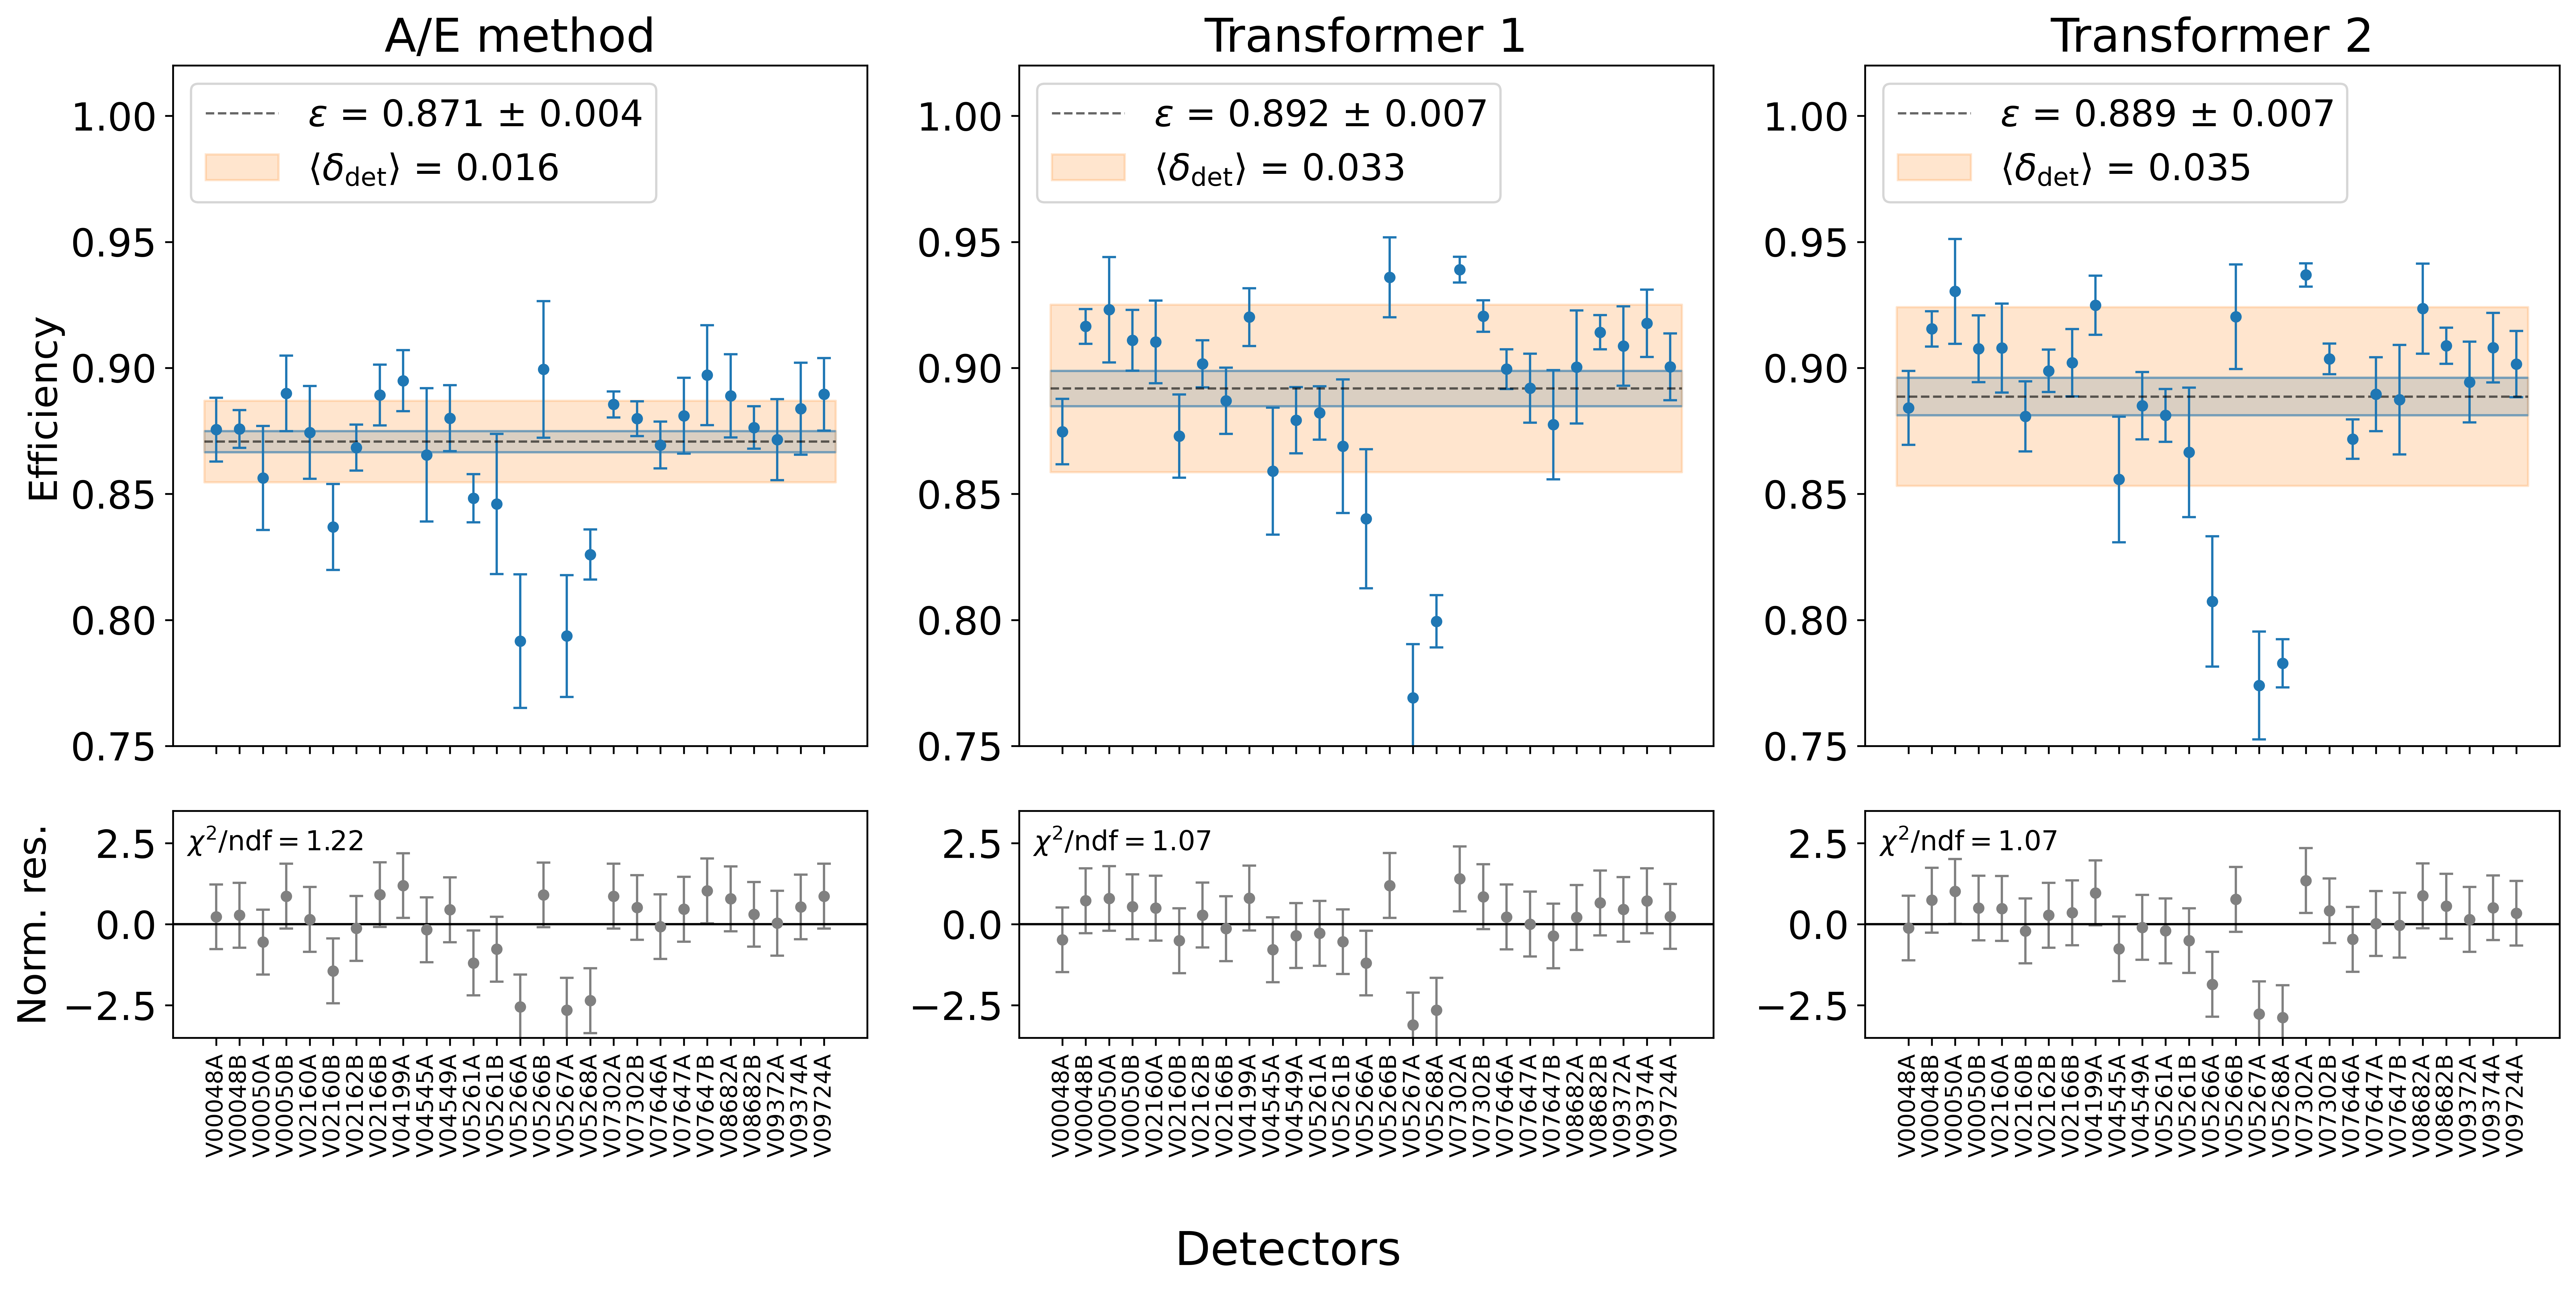
\includegraphics[width=\linewidth]{figures/05_PSD/PSD_eff_DEP_Tl_new.png}
    \caption{PSD efficiencies in the $^{208}$Tl DEP (1592.5~keV) for Mirion detectors used in this analysis. Most detectors exhibit efficiencies (blue band) between 85\% and 90\%, although a few show noticeably lower performance across all PSD methods. The additional detector-to-detector uncertainty is indicated by the orange band. The A/E method shows a small spread ($1.6 \%$), while the Transformer classifications exhibit larger systematic variations ($>3\%$). The lower panel shows the normalized residuals, demonstrating the quality of the fit.} 
\label{fig:psd_dep_Tl}
\end{figure}


\begin{figure}[t]
    \centering
    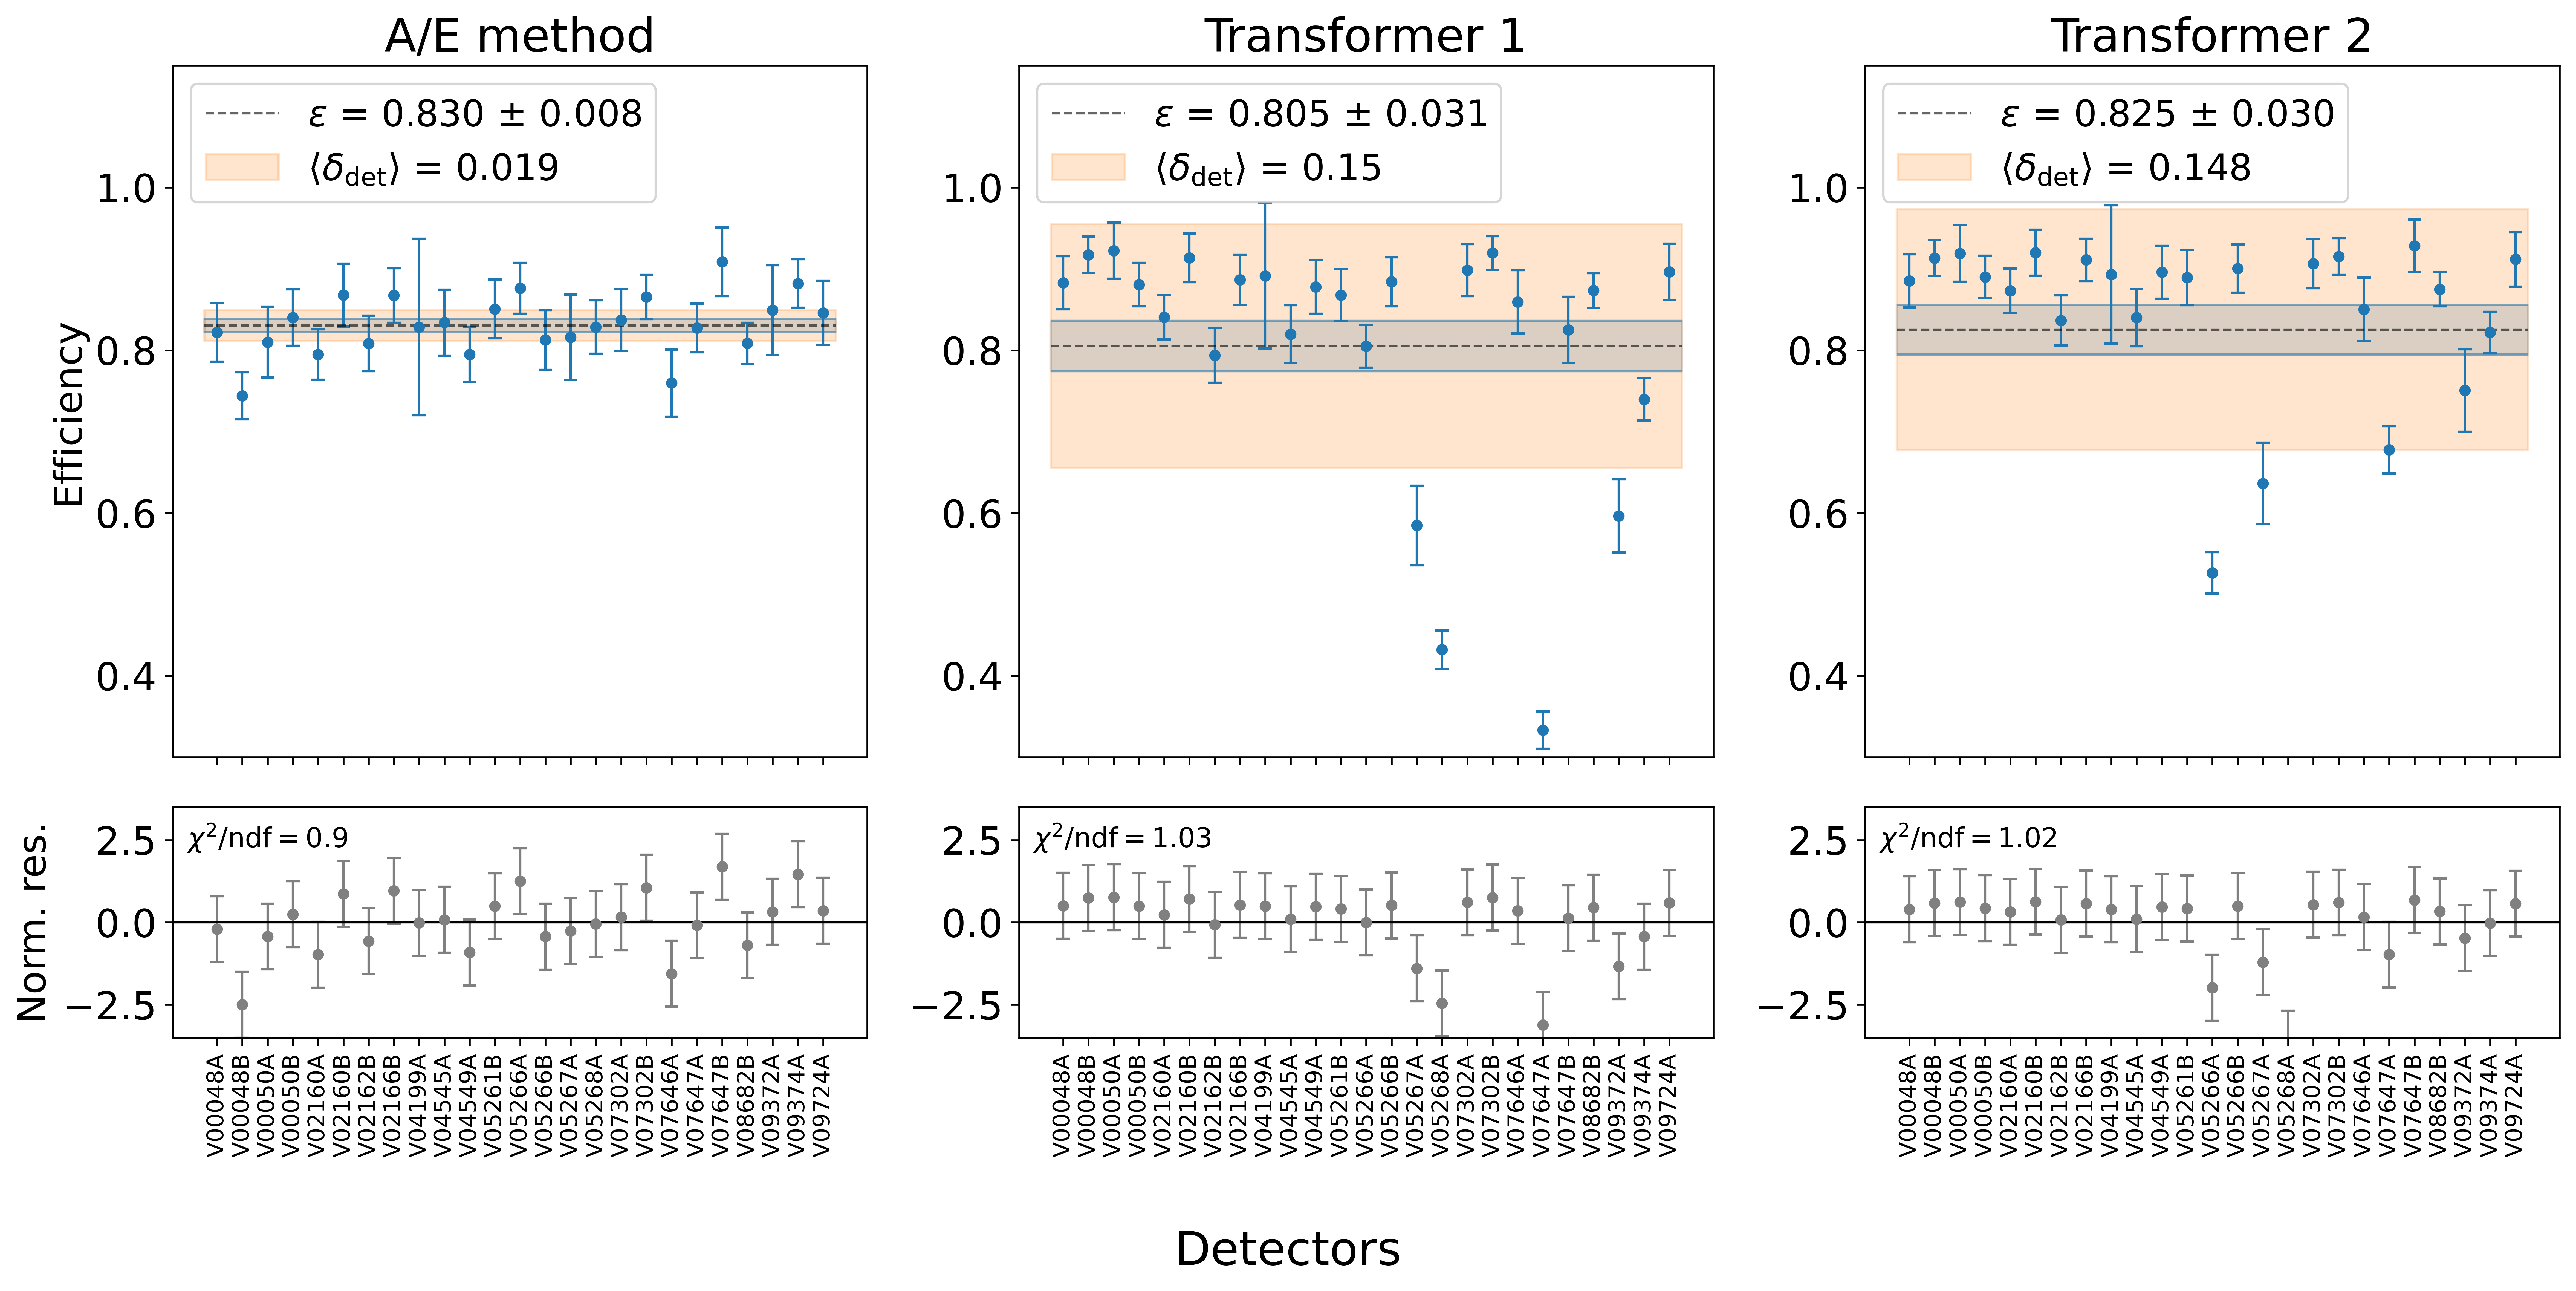
\includegraphics[width=\linewidth]{figures/05_PSD/PSD_eff_DEP_Co_new.png}
    \caption{PSD efficiencies in the $^{56}$Co DEP (2231.5~keV) for Mirion detectors used in this analysis. The efficiency is indicated by the blue band and the detector-to-detector uncertainty by the orange band. The Transformer models show less robustness compared to the A/E method when applied to this DEP. In several detectors, the Transformer classification fails completely. Possible causes include detector-specific waveform variations not captured in training or sensitivity to isotope-dependent event topologies, leading to significantly increased uncertainty. The lower panel shows the normalized residuals, demonstrating the quality of the fit. } 
\label{fig:psd_dep_Co}
\end{figure} 

\begin{table}
\centering
\caption{Additional uncertainty representing unaccounted detector-to-detector variations at the $^{208}$Tl and $^{56}$Co DEPs, and the systematic run-to-run variation. The PSD performance at the $^{208}$Tl DEP exhibits some spread ($< 4\%$). While the efficiency is very stable over time ($< 1\%$ for all models), the Transformer models show a very large detector-to-detector variation.}
\begin{tabular}{||c | c | c | c ||}
	\hline
 	\textbf{Quantity}  & \textbf{A/E [\%]} & \textbf{Model 1 [\%]} & \textbf{Model 2 [\%]} \\
 	\hline
    $\langle \delta_{\mathrm{det}} \rangle$ ($^{228}$Th) & 1.6 & 3.3 & 3.5  \\
 	\hline
 	$\langle \delta_{\mathrm{det}} \rangle$ ($^{56}$Co) & 1.9 & 15.0 & 14.8 \\
    \hline
 	$\langle \delta_{\mathrm{run}} \rangle$ & 0.8 & 0.6 & 0.9 \\ 
    \hline
\end{tabular}
\label{tab:fit_variances}
\end{table}

\subsubsection{Time dependence}

To estimate how the PSD efficiency varies over time across different data-taking periods, we repeat the procedure explained in the previous section. Instead of grouping the data by detector, we now group it by run. Each subset thus contains events from all detectors used in the analysis during that run. 
We then fit the efficiency data per run using the same statistical model, but we reinterpret the additional uncertainty term. In equation~\refeq{eq:chi2_eff_fit}, the detector-specific term $\langle \delta_{\mathrm{det}} \rangle$ is replaced by a run-specific term $\langle \delta_{\mathrm{run}} \rangle$, which quantifies the spread in the efficiencies due to potential time-dependent effects, such as drifts in detector response, electronic noise variations, or changes in environmental conditions.

\begin{equation}
\label{eq:chi2_eff_fit_time}
	\chi^2(\epsilon_i, \sigma_{\epsilon, i} \mid \langle \epsilon \rangle, \langle \delta_{\text{run}} \rangle) =
	\sum_i \left[ \frac{(\epsilon_i - \langle \epsilon \rangle)^2}{\sigma_{\epsilon,i}^2 + \langle \delta_{\text{run}} \rangle^2} + \log(\sigma_{\epsilon,i}^2 + \langle \delta_{\text{run}} \rangle^2) \right] \,.
\end{equation}

This approach allows us to quantify any systematic run-to-run variations in the PSD efficiency. The PSD efficiencies are illustrated in figure~\ref{fig:psd_timevar}, the spread due to time-dependent effects is shown in table~\ref{tab:fit_variances}. 


\begin{figure}
    \centering
    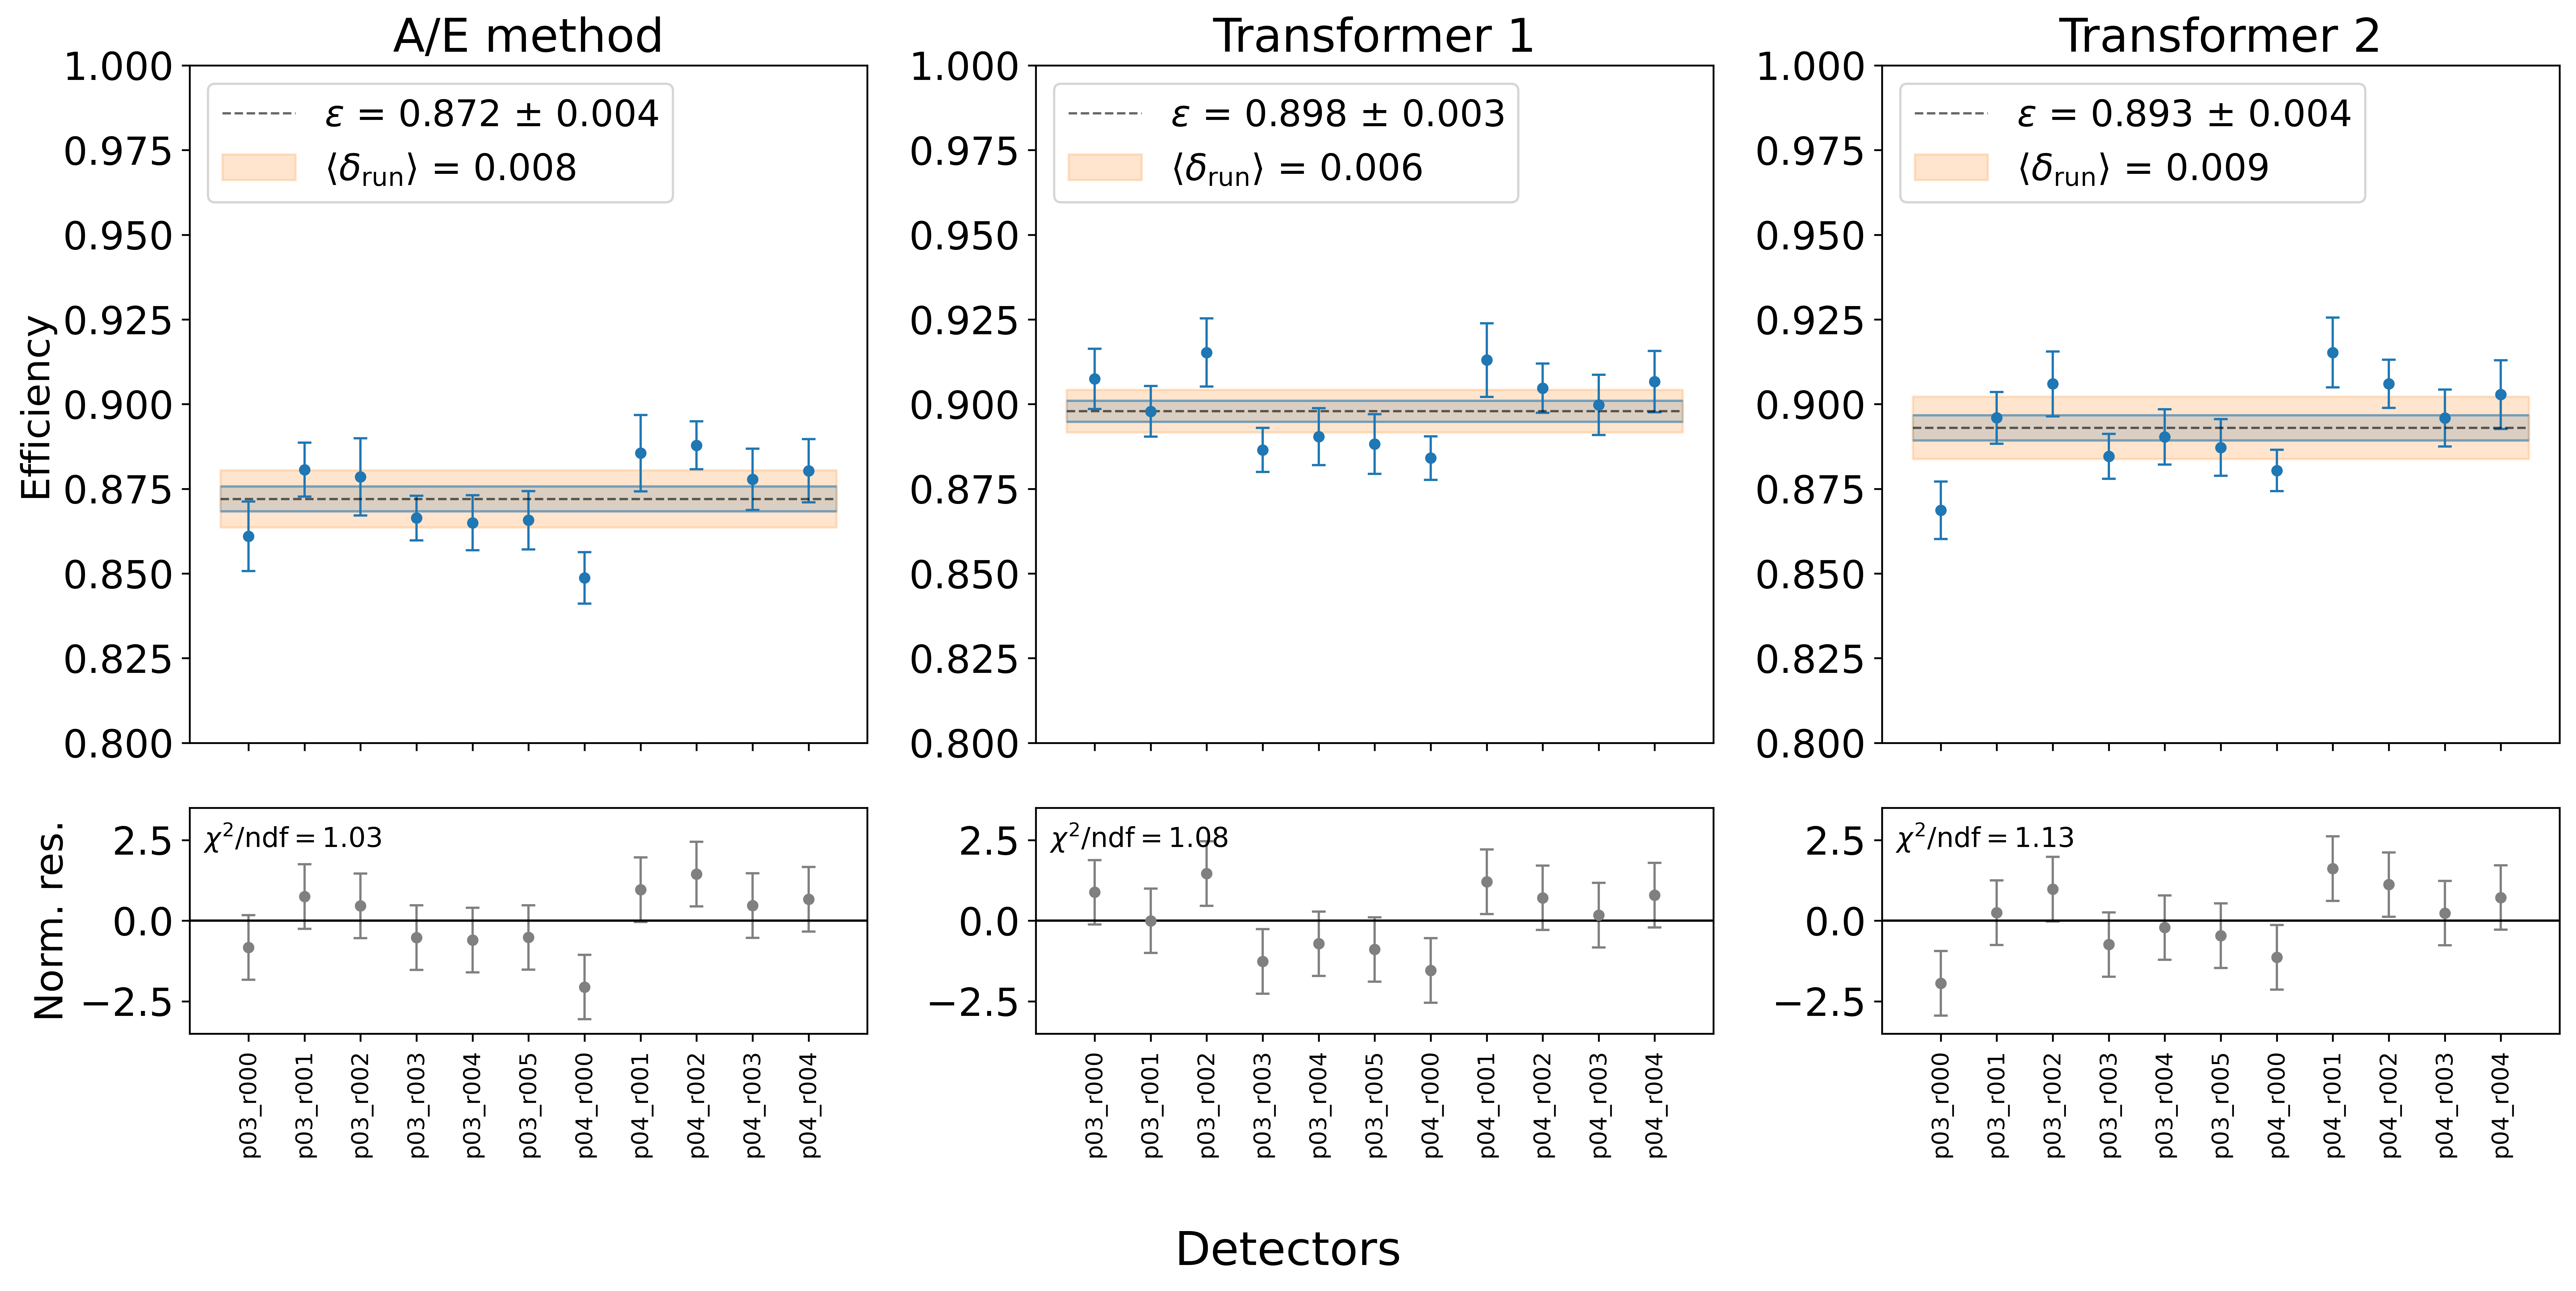
\includegraphics[width=\linewidth]{figures/05_PSD/PSD_eff_timevar_new.png}
    \caption{Time stability of the PSD efficiency (blue band) in the $^{208}$Tl DEP, shown per run for all detectors used. The efficiency remains very stable over time, and there is very little time-dependent uncertainty ($< 1\%$ throughout all models). The bottom panel shows the normalized residuals. }
\label{fig:psd_timevar}
\end{figure}



\subsubsection{Combined efficiency at \texorpdfstring{$Q_{\beta \beta}$}{}}

Although the $^{56}$Co source produces several higher-energy DEPs, most exhibit limited statistics and are therefore not suitable for a reliable estimation of the PSD efficiency estimates. 
To estimate the PSD efficiency at the region of interest, $\epsilon_{Q_{\beta \beta}}$, we perform a linear fit to the PSD efficiencies measured at the three selected energy regions. This is shown in figure~\ref{fig:psd_eff_qbb}. The uncertainty is obtained by propagating the uncertainties from the fit parameters using the covariance matrix:

\begin{equation}
\label{eq:linear_with_unc}
	\sigma_{\epsilon_{Q_{\beta \beta}}} = J \cdot \mathrm{Cov} \cdot J^\intercal \, ,
\end{equation}

\noindent where $J = \left[ \frac{\partial y}{\partial a} \; \frac{\partial y}{\partial b}\right]$ is the Jacobian and $\mathrm{Cov}$ the covariance matrix of the fitted parameters. 


\begin{figure}
    \centering
    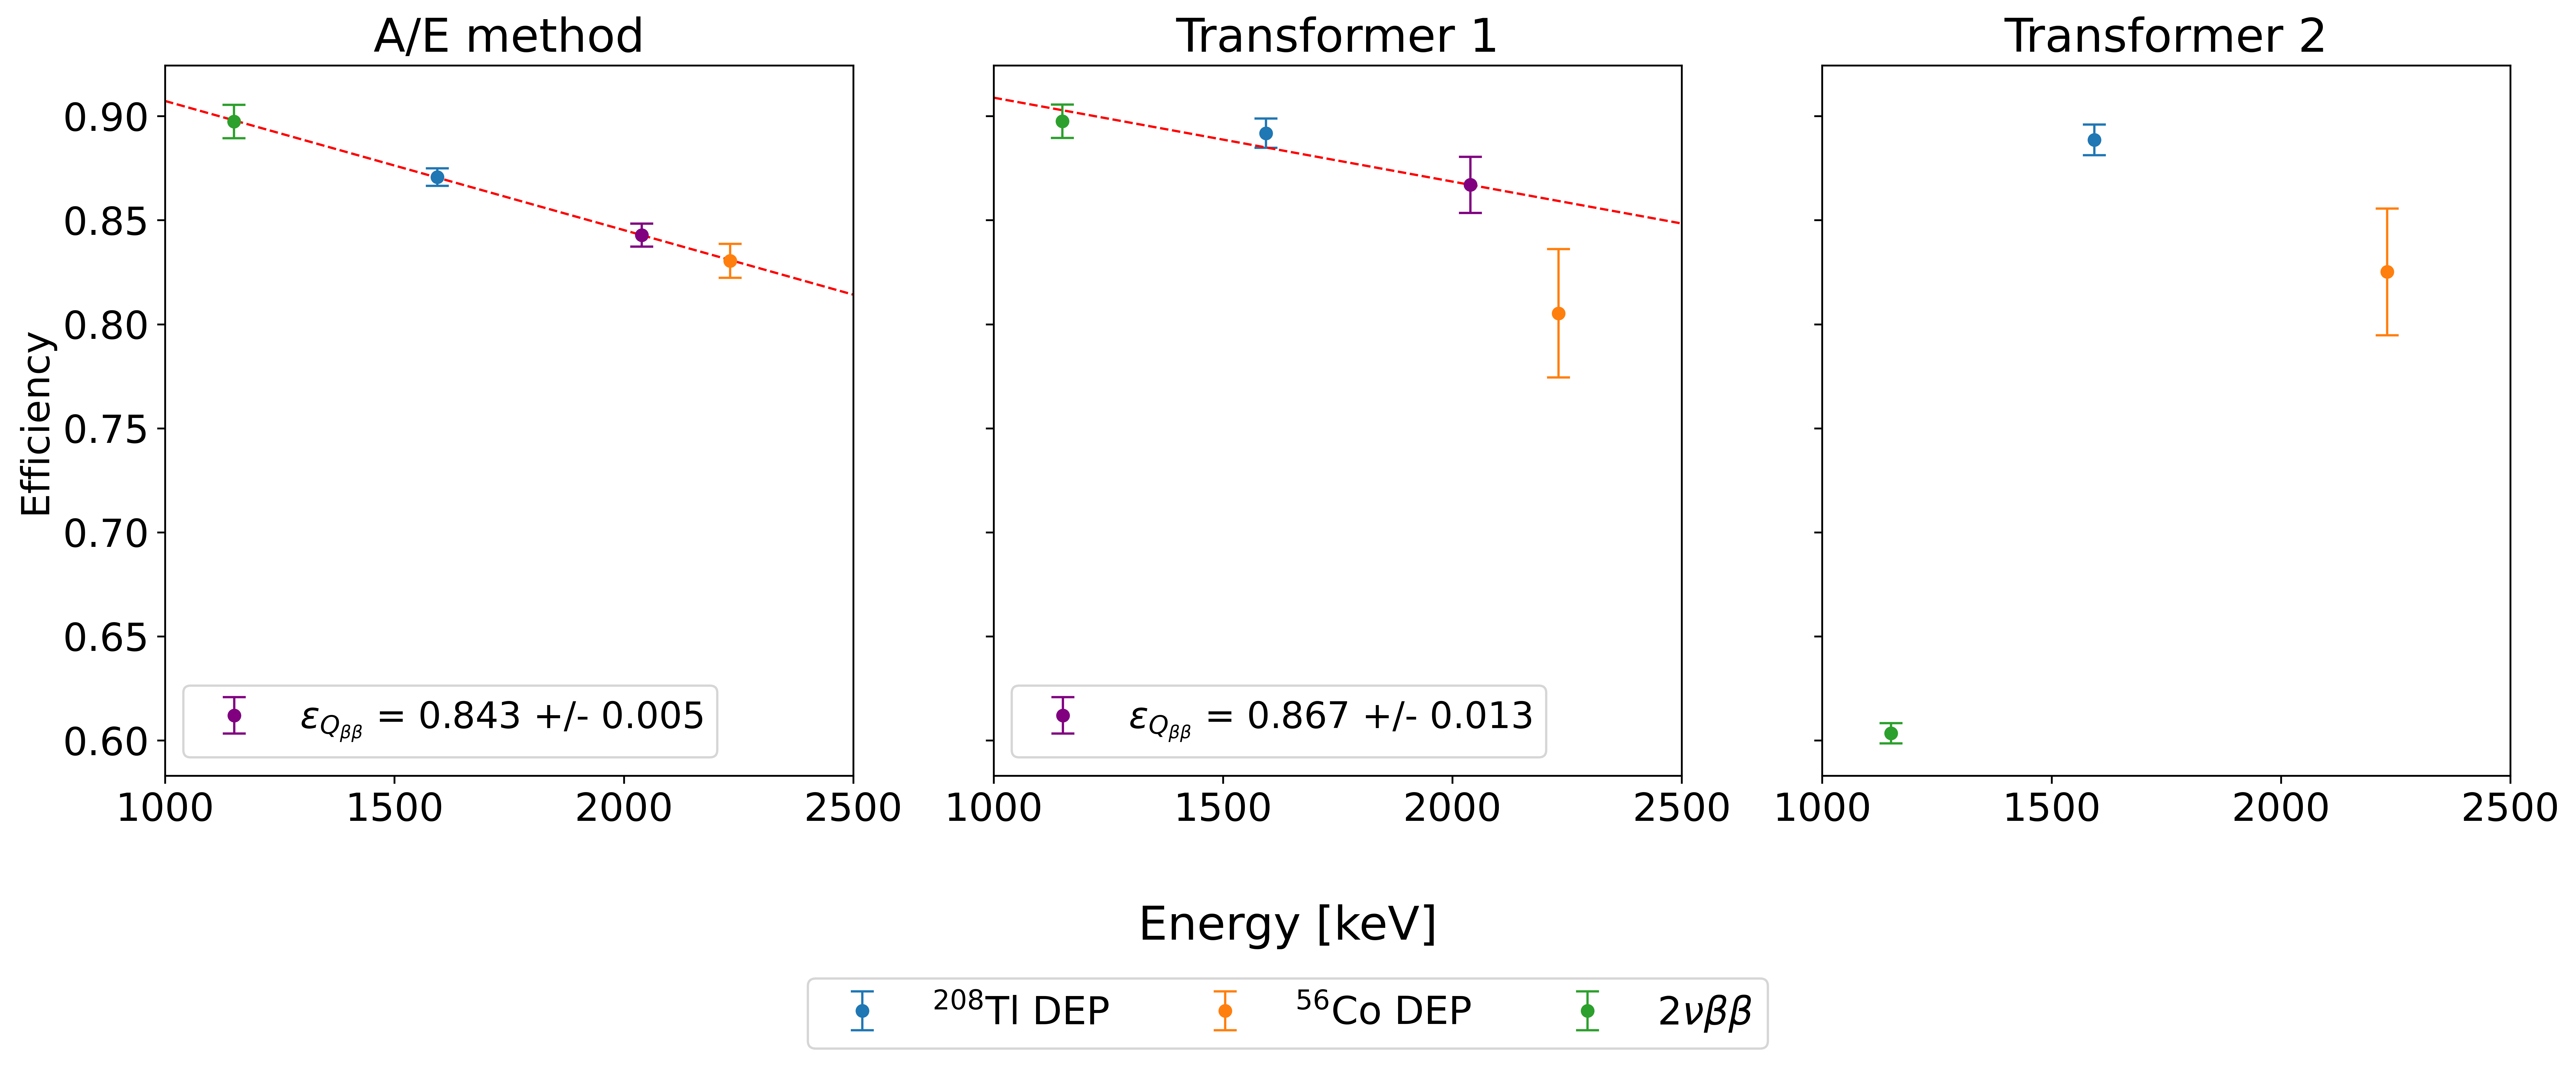
\includegraphics[width=\linewidth]{figures/05_PSD/PSD_eff_qbb.png}
    \caption{PSD efficiency as a function of energy for the three PSD methods. We evaluate the PSD efficiency at three different energies and extrapolate to $Q_{\beta \beta}$ using a linear fit. The A/E method is the most precise. The PSD efficiency of Transformer 1 is higher but exhibits a larger uncertainty. The Transformer model 2 failed for the $2 \nu \beta \beta$ decay events, which is why no fit was performed.}
\label{fig:psd_eff_qbb}
\end{figure}


The combined experimental efficiency of the experiment $\epsilon$, which enters the Bayesian fit as a nuisance parameter, includes also the liquid argon veto efficiency $\epsilon_{\mathrm{LAr}}$, the quality cut efficiency $\epsilon_{\mathrm{quality}}$, the fraction of active detector mass $\epsilon_{\mathrm{active}}$ and the $^{76}$Ge enrichment fraction $\epsilon_{\mathrm{Ge}}$. 
Therefore, the total experimental efficiency is given by:

\begin{equation}
\label{eq:total_efficiency}
	\epsilon = \epsilon_{\mathrm{PSD}} \cdot \epsilon_{\mathrm{LAr}} \cdot \epsilon_{\mathrm{quality}} \cdot \epsilon_{\mathrm{active}} \cdot \epsilon_{\mathrm{Ge}} \, .
\end{equation}

The associated uncertainty is estimated using Gaussian error propagation. Factoring out the total efficiency $\epsilon$, we find:  

\begin{equation}
\label{eq:total_efficiency_unc}
	\sigma_{\epsilon} = \epsilon \cdot \sqrt{ \sum_i \left( \frac{\sigma_{\epsilon_i}}{\epsilon_i} \right) } \, ,
\end{equation}

\noindent where the sum runs over all individual efficiency contributions listed above. The experimental efficiencies, not including PSD efficiencies, are summarized in table~\ref{tab:exp_effs}. These values were obtained from the LEGEND-200 internal metadata database, which is maintained by the collaboration and not publicly released. Efficiencies are provided for each detector and data-taking period; in this analysis, only periods 3 and 4 are used. For each efficiency type, the per-detector values were combined into a single number by taking the arithmetic mean, with the uncertainty given by the standard error of the mean.

\begin{table}
\centering
\caption{Summary of non-PSD experimental efficiencies in the range around $Q_{\beta \beta}$ used in this analysis. Values are taken from the LEGEND-200 internal metadata database for periods 3 and 4 only. For each efficiency type, the per-detector values were averaged, and the quoted uncertainty is the standard error of the mean across detectors.}
\begin{tabular}{||c | c ||}
	\hline
 	\textbf{Efficiency}  & \textbf{Value [\%]} \\
 	\hline
	Liquid Argon veto & $93 \pm 1$  \\
 	\hline
 	Quality cuts & $97.48 \pm 0.01$ \\
 	\hline
 	Active volume & $ 92.5 \pm 0.3 $ \\
 	\hline
 	$^{76}$Ge enrichment & $ 92.6 \pm 0.1$ \\
 	\hline
	Total (excluding PSD) & $77.7 \pm 0.9$ \\
	\hline
\end{tabular}
\label{tab:exp_effs}
\end{table}



\subsection{Pulse shape simulation}

The LEGEND-200 collaboration began developing a software package called LegendGeSim~\cite{noauthor_legend-explegendgesimjl_2025} with the goal of simulating detector waveforms for comparison studies with real data. 
This pulse shape simulation (PSS) framework is intended to support the validation of signal processing, and the goal was to use it to increase event classification across different energies. 
Written in Julia, LegendGeSim generates both idealized and partly realistic waveforms starting with a Geant4 simulation output. 
These results are stored in so-called PET files, which contain event position, energy and time information needed to simulate charge collection and signal formation in germanium detectors. The detector geometries required for these simulations are provided through metadata. 

The PET files are produced using ReMaGe, a modern \texttt{C\kern-.05em\texttt{++}} Geant4-based simulation framework for germanium experiments~\cite{pertoldi_remage_2025}. The geometries themselves are defined in the legend-pygeom-l200 package~\cite{noauthor_legend-explegend-pygeom-l200_2025}, developed within the LEGEND-200 collaboration. 
Finally, a dedicated interface script was developed to convert the Geant4 output into a format compatible with LegendGeSim. Additionally, a coordinate transformation is required, since ReMaGe and LegendGeSim use different coordinate systems\footnote{Credit to Giovanna Saleh for identifying and resolving this inconsistency.}.  

Figure~\ref{fig:PSS_diagram} illustrates the interaction between the various software components used in the waveform simulation pipeline. 

\begin{figure}
\centering
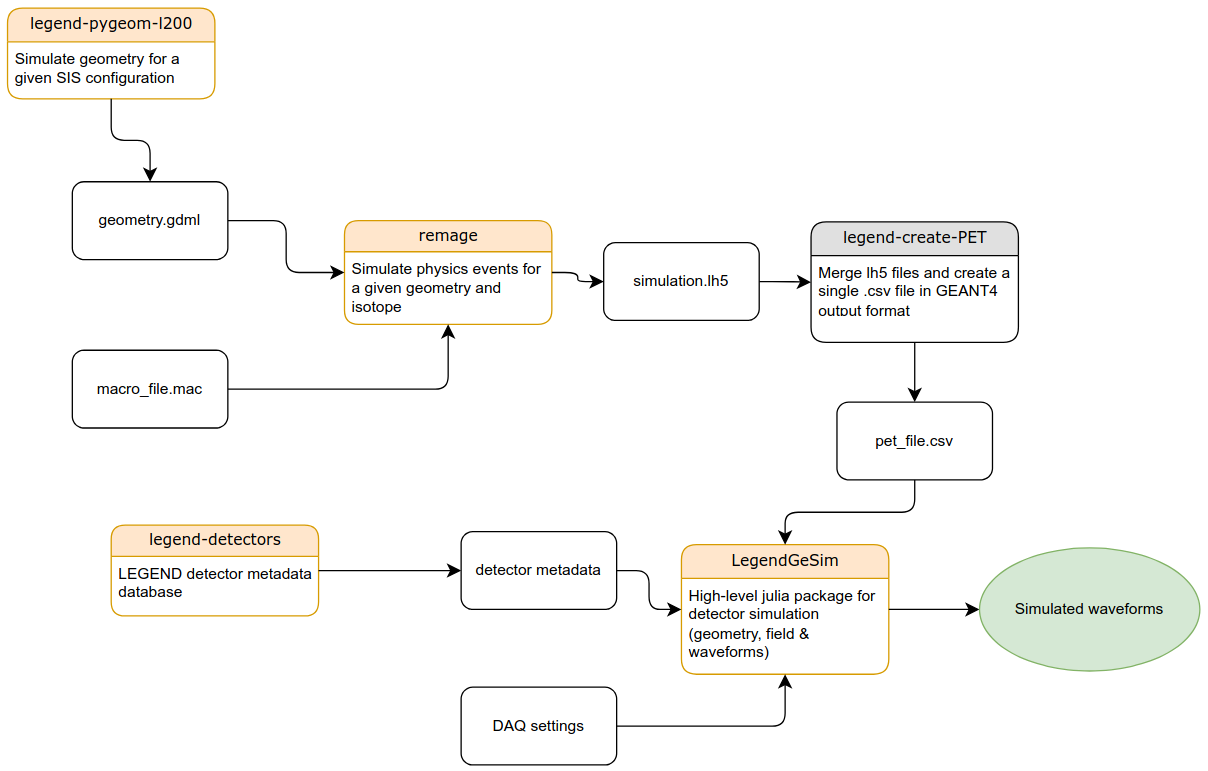
\includegraphics[width=\linewidth]{figures/05_PSD/PSS_diagram.png}
\caption{Connection between different LEGEND packages for the use of LegendGeSim.} 
\label{fig:PSS_diagram}
\end{figure}

Despite the promising concept, the LegendGeSim framework remains under development and is not yet fully functional. In attempting to use it, we encountered several limitations that hindered its use for this project: 
\begin{itemize}
\item \textbf{Incomplete physics modeling}: Essential mechanisms such as diffusion, charge cloud drift, charge trapping, and temperature dependence are either not fully implemented or not comparable with data.  
\item \textbf{Systematic uncertainties}: Systematics associated with different PSD parameters and the simulated electronics chain are not yet characterized. 
\item \textbf{Inaccurate energy reconstruction}: The trapezoidal filter used in the framework systematically underestimates the true energy of events. 
\end{itemize}

The inaccurate energy reconstruction is evident in figure~\ref{fig:PSS_histogram}, which compares simulated data to calibration measurements. Example waveforms are shown in figure~\ref{fig:PSS_waveforms}, where a systematic slowly rising current signal is visible.  

The current pulse shape simulation workflow suffers from significant inefficiency, with runtimes so long that large-scale waveform generation is impractical. 
A major bottleneck is that, in its present implementation, ReMaGe must fully simulate each event before deciding whether to retain it. Consequently, complete decay chains (e.g., the $^{228}$Th chain) are simulated, and the full energy spectrum is generated, including events outside the peaks of interest. 
There is the option to restrict the decay chain (e.g., to only $^{208} \mathrm{Tl} \rightarrow ^{208} \mathrm{Pb}$); this has to be handled with care, as it might introduce bias. While it is possible to apply generator-level energy cuts, this approach is non-trivial. These inefficiencies occur before the actual pulse-shape simulation in LegendGeSim. 
For the dataset shown in figure~\ref{fig:PSS_histogram}, the simulation required 27.5~hours of wall time on NERSC (using 128 CPU cores in parallel for ReMaGe only) for a single detector (V09372A), yielding approximately 5000 events in the $^{208}$Tl DEP.  

\begin{figure}
\centering
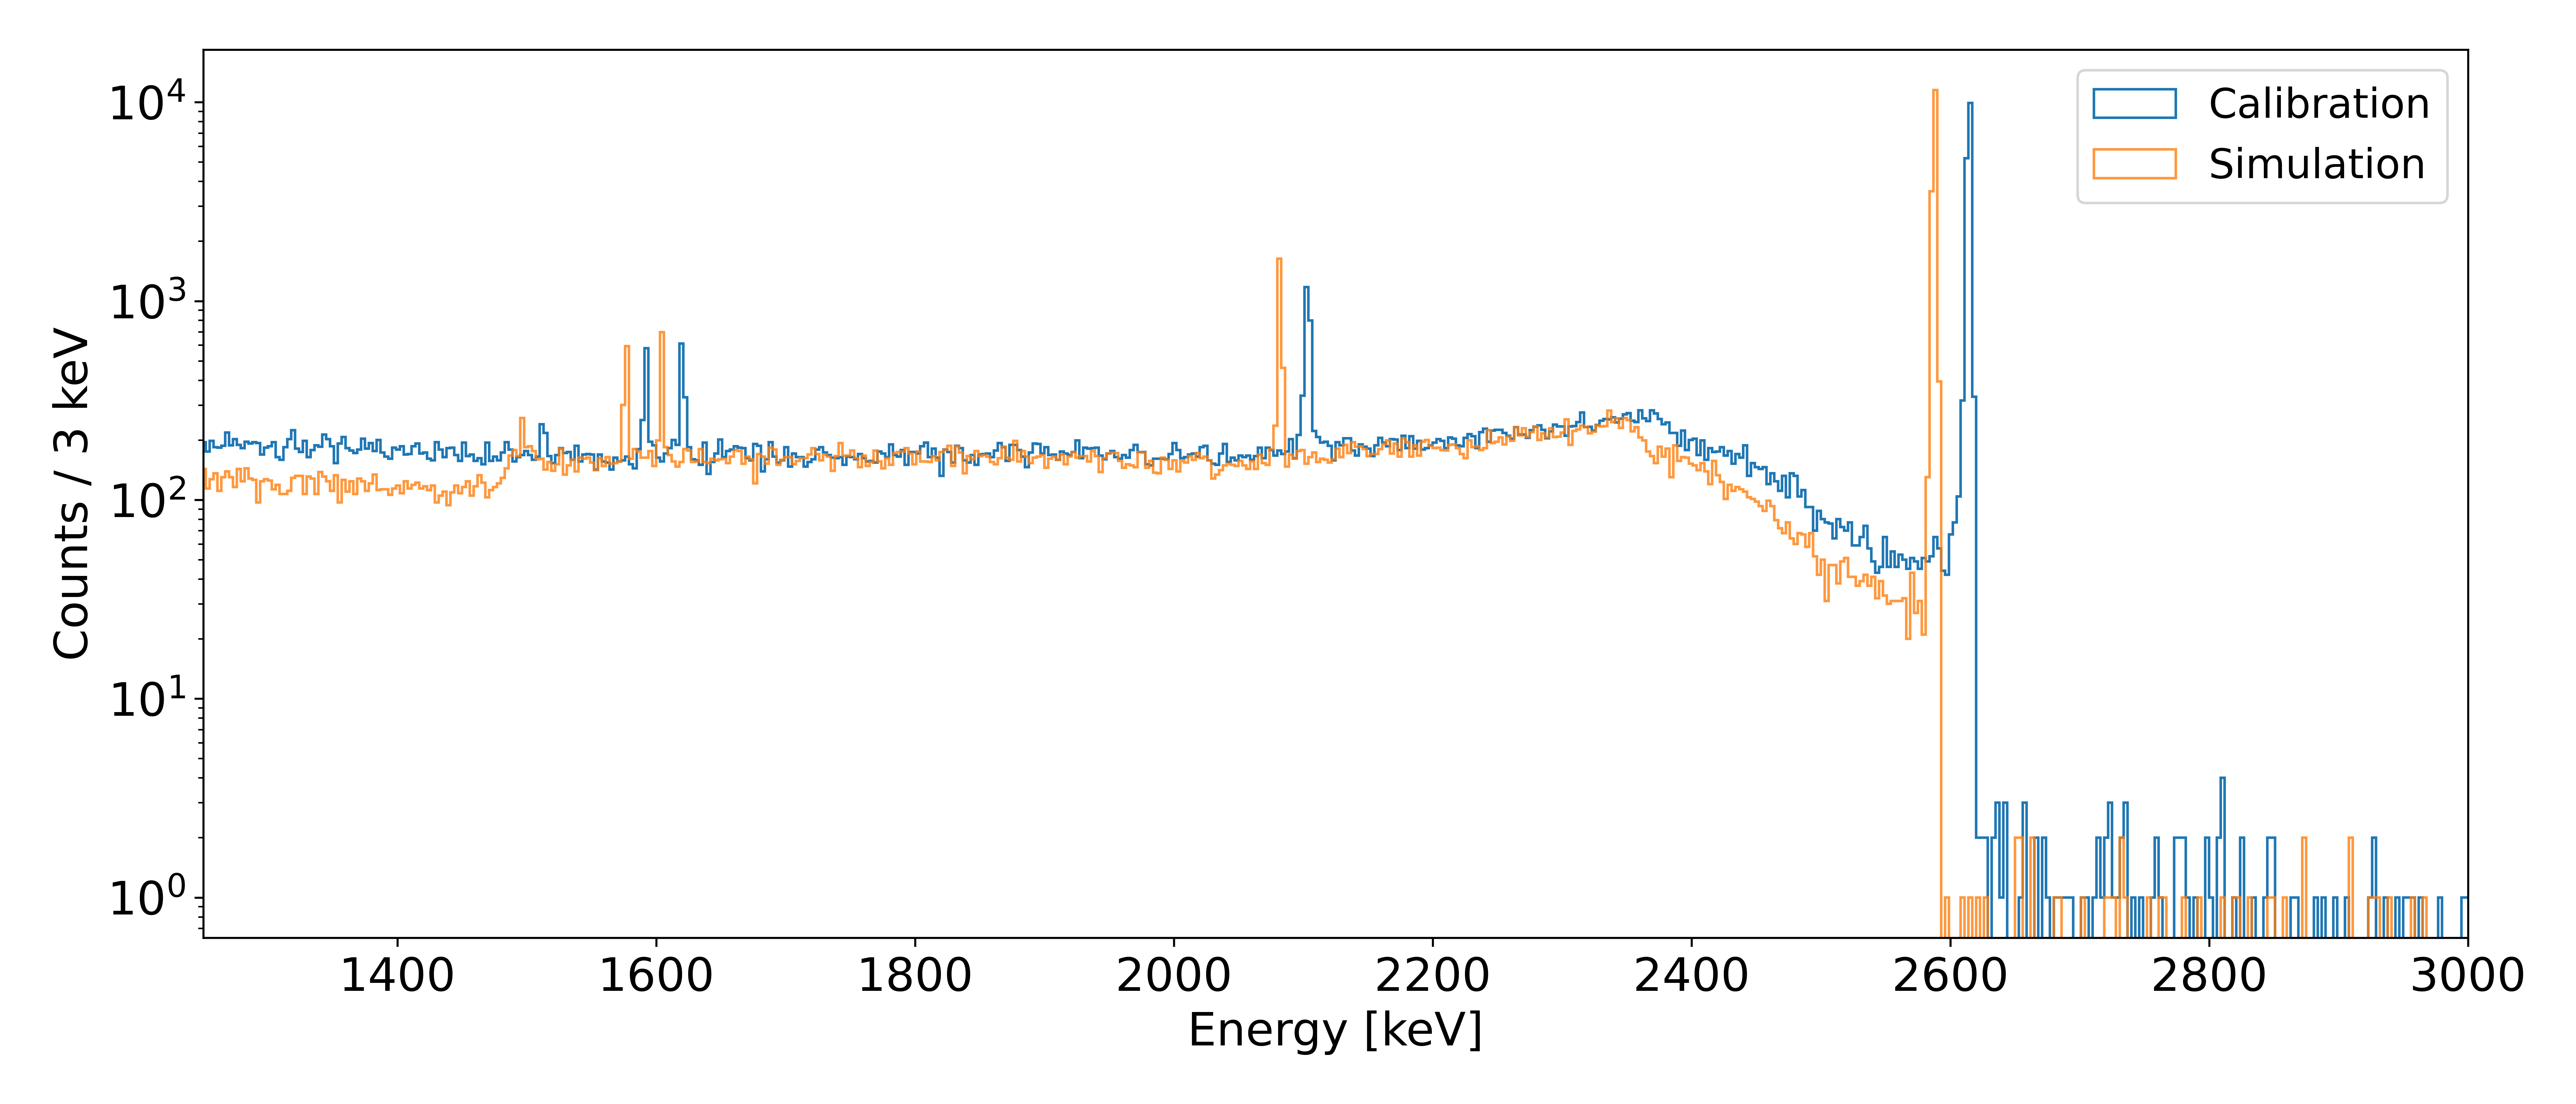
\includegraphics[width=\linewidth]{figures/05_PSD/Plot_cal_vs_PSS.png}
\caption{Energy spectrum for the IC detector V09372A, comparing calibration data (blue) from period 3 with simulated data (orange). In the simulation, the decay chain is restricted to nuclei with $208 \leq A \leq 212$ and $81 \leq Z \leq 83$, and only events with energies above 1200~keV are retained. The simulated spectrum shows a systematic shift of the characteristic $\gamma$-lines toward lower energies, indicating inaccuracies in the energy reconstruction.}
\label{fig:PSS_histogram}
\end{figure}

\begin{figure}
\centering
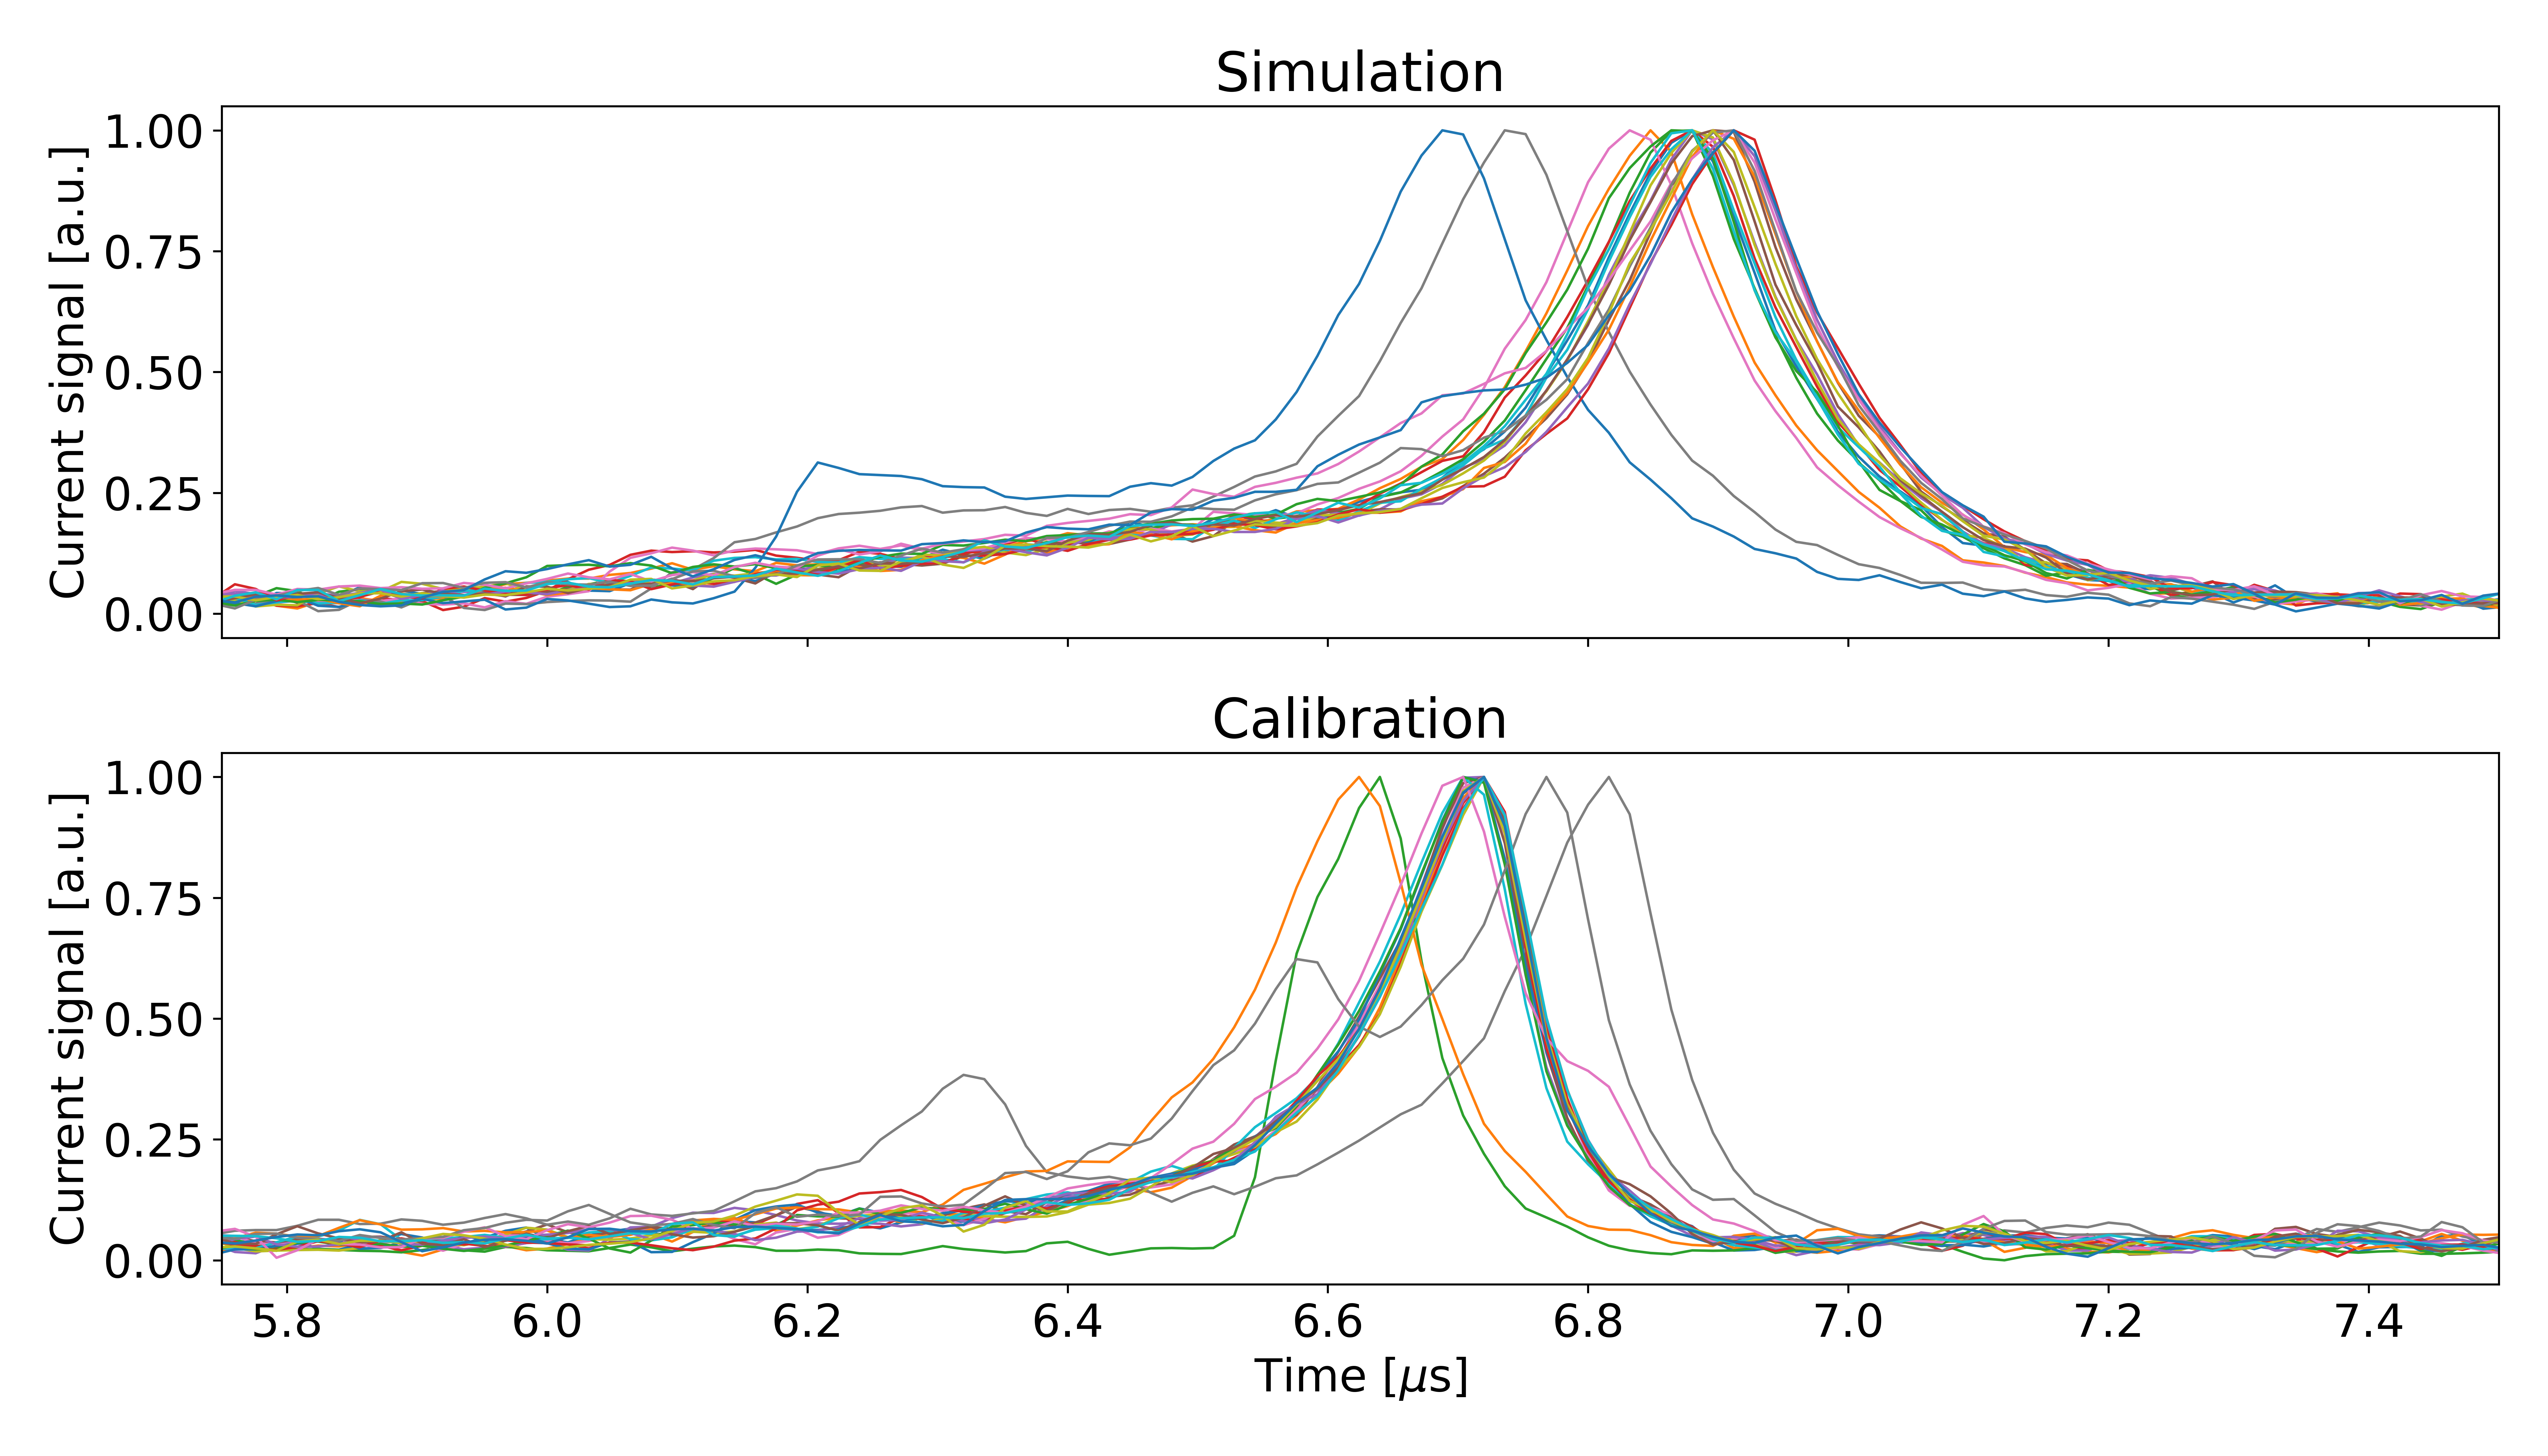
\includegraphics[width=\linewidth]{figures/05_PSD/Plot_waveform_cal_vs_pss.png}
\caption{Example waveforms for the IC detector V09372A in the $^{208}$Tl DEP at 1592.5~keV, comparing simulated waveforms (top panel) with calibration data from period 3 (bottom panel). The simulated waveforms exhibit a systematically slower, early rise compared to the measured data. }
\label{fig:PSS_waveforms}
\end{figure}

The Pulse Shape Simulation (PSS) framework was expected to serve as a practical tool for this study. 
Although some development work was anticipated, the framework turned out to be less mature and more complex to integrate than expected. 
At the time of writing, further development is ongoing within the LEGEND-200 collaboration, with significant contributions from the University of Zurich.
Nonetheless, this work established a functioning processing pipeline for handling simulated PSS data from a single detector. 
Due to time constraints, a full-scale simulation was not achieved, but the essential tools required for generating, processing, and analyzing simulated waveforms are now in place for use in future studies. 




\subsection{Summary and combined results at \texorpdfstring{$Q_{\beta \beta}$}{}}

In this work, a Transformer-based PSD method for the LEGEND-200 experiment was developed. Of the three transformer models tested, only Transformer model 1 demonstrated stable and reliable performance across the full energy range. The PSD efficiency at $Q_{\beta \beta}$ was obtained by interpolating between three reference points: $2 \nu \beta \beta$ decay events in the 1000-1300~keV interval, the 1592.5~keV DEP of $^{208}$Tl, and the 2231.5~keV DEP of $^{56}$Co. Additional systematic uncertainty was included to account for time-dependent stability, detector-to-detector variations, and differences in PSD acceptance between $2 \nu \beta \beta$ and DEP events. The final PSD efficiency yields $(86.7 \pm 1.3)$\% at $Q_{\beta \beta}$ for the Transformer. This is consistent with the efficiency obtained by the conventional A/E method, $(84.3 \pm 0.5)$\%, with a two-sided p-value of $p = 0.08$ indicating no significant difference between the two approaches at the 5\% level. 
Taking into account the experimental efficiencies listed in table~\ref{tab:exp_effs}, the overall detection efficiency achieved with the Transformer-based approach is $(66.8 \pm 2.1)$\%, compared to $(65.0 \pm 2.0)$\% for the A/E method. 